\documentclass[dvipdfmx]{ehis}
%DIF LATEXDIFF DIFFERENCE FILE
%DIF DEL paper_his_original_submitted.tex   Sun Apr 26 12:44:05 2026
%DIF ADD paper_his_revision.tex             Wed Jul  8 12:33:46 2026
\usepackage{graphicx}

\usepackage{amsmath,amssymb,amsfonts}
\usepackage{algorithmic}
\usepackage{textcomp}
\usepackage{xcolor}
\usepackage{url}
\usepackage{booktabs}
\usepackage[caption=false]{subfig}
\usepackage{multirow}
\usepackage{algorithm}
\usepackage{algorithmic}
\usepackage{listings}
\lstdefinelanguage{JavaScript}{
  keywords={const, let, var, function, return, if, else, for, while, switch, case, break, try, catch, finally, window, camerala_logger},
  sensitive=true,
  comment=[l]{//},
  morecomment=[s]{/*}{*/},
  morestring=[b]\",
  morestring=[b]\'
}
%DIF 23-24c23-24
%DIF < \lstdefinelanguage{json}{
%DIF <   morestring=[b]\",
%DIF -------
\lstdefinelanguage{csv}{ %DIF > 
  morecomment=[l]{\#}, %DIF > 
%DIF -------
}

\newcommand{\etal}{\textit{et al.}}
\newcommand{\ie}{\textit{i.e.}}
\newcommand{\eg}{\textit{e.g.}}

%DIF 31c31
%DIF < \etitle{Camerala: A Privacy-Preserving Browser-Native Framework for In-the-Wild Physiological Sensing and Task Measurement}
%DIF -------
\etitle{Camerala: A Local-First Browser-Native Framework for Remote Psychophysiological Task Sensing} %DIF > 
%DIF -------

\eauthor{
Kotaro Furukawa\thanks{College of Transdisciplinary Sciences for Innovation, Kanazawa University, Japan}
}

\YEAR{}
\VOL{}
\NO{}
\TYPE{}


\lstset{
  basicstyle=\ttfamily\scriptsize,
  breaklines=true,
  columns=fullflexible,
  keepspaces=true
}
\makeatletter
\def\@oddhead{}
\def\@evenhead{}
\def\ps@vr{
 \def\@oddhead{}
 \def\@evenhead{}
}
\def\ps@his{
 \def\@oddhead{}
 \def\@evenhead{}
}
\makeatother
%DIF PREAMBLE EXTENSION ADDED BY LATEXDIFF
%DIF UNDERLINE PREAMBLE %DIF PREAMBLE
\RequirePackage[normalem]{ulem} %DIF PREAMBLE
\RequirePackage{color}\definecolor{RED}{rgb}{1,0,0}\definecolor{BLUE}{rgb}{0,0,1} %DIF PREAMBLE
\providecommand{\DIFadd}[1]{{\protect\color{blue}\uwave{#1}}} %DIF PREAMBLE
\providecommand{\DIFdel}[1]{{\protect\color{red}\sout{#1}}} %DIF PREAMBLE
%DIF SAFE PREAMBLE %DIF PREAMBLE
\providecommand{\DIFaddbegin}{} %DIF PREAMBLE
\providecommand{\DIFaddend}{} %DIF PREAMBLE
\providecommand{\DIFdelbegin}{} %DIF PREAMBLE
\providecommand{\DIFdelend}{} %DIF PREAMBLE
\providecommand{\DIFmodbegin}{} %DIF PREAMBLE
\providecommand{\DIFmodend}{} %DIF PREAMBLE
%DIF FLOATSAFE PREAMBLE %DIF PREAMBLE
\providecommand{\DIFaddFL}[1]{\DIFadd{#1}} %DIF PREAMBLE
\providecommand{\DIFdelFL}[1]{\DIFdel{#1}} %DIF PREAMBLE
\providecommand{\DIFaddbeginFL}{} %DIF PREAMBLE
\providecommand{\DIFaddendFL}{} %DIF PREAMBLE
\providecommand{\DIFdelbeginFL}{} %DIF PREAMBLE
\providecommand{\DIFdelendFL}{} %DIF PREAMBLE
\providecommand{\DIFscaledelfig}{0.5}
%DIF HIGHLIGHTGRAPHICS PREAMBLE %DIF PREAMBLE
\RequirePackage{settobox} %DIF PREAMBLE
\RequirePackage{letltxmacro} %DIF PREAMBLE
\newsavebox{\DIFdelgraphicsbox} %DIF PREAMBLE
\newlength{\DIFdelgraphicswidth} %DIF PREAMBLE
\newlength{\DIFdelgraphicsheight} %DIF PREAMBLE
% store original definition of \includegraphics %DIF PREAMBLE
\LetLtxMacro{\DIFOincludegraphics}{\includegraphics} %DIF PREAMBLE
\providecommand{\DIFaddincludegraphics}[2][]{{\color{blue}\fbox{\DIFOincludegraphics[#1]{#2}}}} %DIF PREAMBLE
\providecommand{\DIFdelincludegraphics}[2][]{% %DIF PREAMBLE
\sbox{\DIFdelgraphicsbox}{\DIFOincludegraphics[#1]{#2}}% %DIF PREAMBLE
\settoboxwidth{\DIFdelgraphicswidth}{\DIFdelgraphicsbox} %DIF PREAMBLE
\settoboxtotalheight{\DIFdelgraphicsheight}{\DIFdelgraphicsbox} %DIF PREAMBLE
\scalebox{\DIFscaledelfig}{% %DIF PREAMBLE
\parbox[b]{\DIFdelgraphicswidth}{\usebox{\DIFdelgraphicsbox}\\[-\baselineskip] \rule{\DIFdelgraphicswidth}{0em}}\llap{\resizebox{\DIFdelgraphicswidth}{\DIFdelgraphicsheight}{% %DIF PREAMBLE
\setlength{\unitlength}{\DIFdelgraphicswidth}% %DIF PREAMBLE
\begin{picture}(1,1)% %DIF PREAMBLE
\thicklines\linethickness{2pt} %DIF PREAMBLE
{\color[rgb]{1,0,0}\put(0,0){\framebox(1,1){}}}% %DIF PREAMBLE
{\color[rgb]{1,0,0}\put(0,0){\line( 1,1){1}}}% %DIF PREAMBLE
{\color[rgb]{1,0,0}\put(0,1){\line(1,-1){1}}}% %DIF PREAMBLE
\end{picture}% %DIF PREAMBLE
}\hspace*{3pt}}} %DIF PREAMBLE
} %DIF PREAMBLE
\LetLtxMacro{\DIFOaddbegin}{\DIFaddbegin} %DIF PREAMBLE
\LetLtxMacro{\DIFOaddend}{\DIFaddend} %DIF PREAMBLE
\LetLtxMacro{\DIFOdelbegin}{\DIFdelbegin} %DIF PREAMBLE
\LetLtxMacro{\DIFOdelend}{\DIFdelend} %DIF PREAMBLE
\DeclareRobustCommand{\DIFaddbegin}{\DIFOaddbegin \let\includegraphics\DIFaddincludegraphics} %DIF PREAMBLE
\DeclareRobustCommand{\DIFaddend}{\DIFOaddend \let\includegraphics\DIFOincludegraphics} %DIF PREAMBLE
\DeclareRobustCommand{\DIFdelbegin}{\DIFOdelbegin \let\includegraphics\DIFdelincludegraphics} %DIF PREAMBLE
\DeclareRobustCommand{\DIFdelend}{\DIFOaddend \let\includegraphics\DIFOincludegraphics} %DIF PREAMBLE
\LetLtxMacro{\DIFOaddbeginFL}{\DIFaddbeginFL} %DIF PREAMBLE
\LetLtxMacro{\DIFOaddendFL}{\DIFaddendFL} %DIF PREAMBLE
\LetLtxMacro{\DIFOdelbeginFL}{\DIFdelbeginFL} %DIF PREAMBLE
\LetLtxMacro{\DIFOdelendFL}{\DIFdelendFL} %DIF PREAMBLE
\DeclareRobustCommand{\DIFaddbeginFL}{\DIFOaddbeginFL \let\includegraphics\DIFaddincludegraphics} %DIF PREAMBLE
\DeclareRobustCommand{\DIFaddendFL}{\DIFOaddendFL \let\includegraphics\DIFOincludegraphics} %DIF PREAMBLE
\DeclareRobustCommand{\DIFdelbeginFL}{\DIFOdelbeginFL \let\includegraphics\DIFdelincludegraphics} %DIF PREAMBLE
\DeclareRobustCommand{\DIFdelendFL}{\DIFOaddendFL \let\includegraphics\DIFOincludegraphics} %DIF PREAMBLE
%DIF AMSMATHULEM PREAMBLE %DIF PREAMBLE
\makeatletter %DIF PREAMBLE
\let\sout@orig\sout %DIF PREAMBLE
\renewcommand{\sout}[1]{\ifmmode\text{\sout@orig{\ensuremath{#1}}}\else\sout@orig{#1}\fi} %DIF PREAMBLE
\makeatother %DIF PREAMBLE
%DIF COLORLISTINGS PREAMBLE %DIF PREAMBLE
\RequirePackage{listings} %DIF PREAMBLE
\RequirePackage{color} %DIF PREAMBLE
\lstdefinelanguage{DIFcode}{ %DIF PREAMBLE
%DIF DIFCODE_UNDERLINE %DIF PREAMBLE
  moredelim=[il][\color{red}\sout]{\%DIF\ <\ }, %DIF PREAMBLE
  moredelim=[il][\color{blue}\uwave]{\%DIF\ >\ } %DIF PREAMBLE
} %DIF PREAMBLE
\lstdefinestyle{DIFverbatimstyle}{ %DIF PREAMBLE
	language=DIFcode, %DIF PREAMBLE
	basicstyle=\ttfamily, %DIF PREAMBLE
	columns=fullflexible, %DIF PREAMBLE
	keepspaces=true %DIF PREAMBLE
} %DIF PREAMBLE
\lstnewenvironment{DIFverbatim}[1][]{\lstset{style=DIFverbatimstyle}}{} %DIF PREAMBLE
\lstnewenvironment{DIFverbatim*}[1][]{\lstset{style=DIFverbatimstyle,showspaces=true}}{} %DIF PREAMBLE
\lstset{extendedchars=\true,inputencoding=utf8}

%DIF END PREAMBLE EXTENSION ADDED BY LATEXDIFF

\begin{document}

\begin{abstract}
\DIFdelbegin \DIFdel{Continuous physiological sensing and synchronized task measurement in naturalistic environments is challenging. Systems relying on cloud-based video transmission face privacy constraints, while uncontrolled conditions—such as variable lighting, posture, motion, and camera placement—can severely degrade measurement quality and cross-environment comparability. We present Camerala , a privacy-conscious}\DIFdelend \DIFaddbegin \DIFadd{Camerala is a local-first}\DIFaddend , browser-native \DIFdelbegin \DIFdel{sensing framework designed to address these challenges. By utilizing WebAssembly (Wasm) and WebGL backends, the framework extracts remote photoplethysmography (rPPG) and facial landmarks entirely on the client device, avoiding raw video transmission.
Furthermore, it integrates sensing, psychophysical task timing, and local data persistence within a unified client-side runtime.
To evaluate the framework, we conducted an exploratory 10-session longitudinal deployment (}\DIFdelend \DIFaddbegin \DIFadd{framework for remote psychological and psychophysiological task experiments.
It synchronizes task events with face-image-derived feature records and exports local CSV/ZIP files without transmitting or storing raw facial video.
In an exploratory }\DIFaddend N=1 \DIFdelbegin \DIFdel{) across }\DIFdelend \DIFaddbegin \DIFadd{author-participant deployment, ten sessions were conducted in }\DIFaddend laboratory and home settings\DIFaddbegin \DIFadd{, yielding 600 trials in total.
After applying a reaction-time criterion of 100--1500 ms, 541/600 trials remained for descriptive analysis.
The exported logs contained timestamped task events and reproducible face-image-derived fields.
Differences between laboratory and home records are reported as deployment-specific sensor-derived observations, not as evidence of psychological, physiological, cognitive, motivational, or rPPG-accuracy effects}\DIFaddend .
\DIFdelbegin \DIFdel{The deployment showed that the system could operate across diverse physical contexts and that between-environment differences were observable in the resulting physiological signals.
These results suggest that browser-native edge architectures can support deployment-oriented, privacy-conscious physiologicalsensing across heterogeneous home and laboratory environments.
}\DIFdelend \end{abstract}

\begin{keyword}
\DIFdelbegin \DIFdel{WebAssembly}\DIFdelend \DIFaddbegin \DIFadd{Browser-Native Sensing}\DIFaddend , Remote Photoplethysmography, \DIFdelbegin \DIFdel{Browser-Native Sensing, Privacy-Preserving Frameworks, In-the-Wild Deployment
}\DIFdelend \DIFaddbegin \DIFadd{FaceMesh, Local-First Logging, Task-Aligned Measurement, Laboratory and Home Settings
}\DIFaddend \end{keyword}

\maketitle

% =================================================================================
% SECTION 1: INTRODUCTION
% =================================================================================
\section{Introduction}

\DIFdelbegin \DIFdel{Continuous monitoring of physiological signals and task-derived metrics in naturalistic, "in-the-wild" environments provides critical insights for ubiquitous computing and human-computer interaction (HCI).
While medical-grade sensors (e.g., electrocardiograms) succeed in controlled laboratories, deploying sensor systems in domestic environments introduces significant engineering challenges. 
}\DIFdelend \DIFaddbegin \DIFadd{Remote psychological and psychophysiological task experiments often require synchronized behavioral task logs and webcam-derived feature records while avoiding unnecessary handling of privacy-sensitive facial video.
This use case is not unconstrained daily-life sensing: the participant is seated in front of a laptop, views task stimuli, and responds through the browser.
Even in this task-constrained setting, deployment outside a controlled laboratory introduces practical difficulties for human-interface research, including heterogeneous illumination, camera placement, posture, browser timing, and local data handling.
}\DIFaddend 

\DIFdelbegin \DIFdel{First, there are strict privacy constraints. In many practical pipelines, }\DIFdelend \DIFaddbegin \DIFadd{Many }\DIFaddend video-based physiological \DIFdelbegin \DIFdel{analysis relies on external processing }\DIFdelend \DIFaddbegin \DIFadd{measurement pipelines rely on raw video recording }\DIFaddend or server-side \DIFdelbegin \DIFdel{components.
This approach raises privacy concerns, particularly }\DIFdelend \DIFaddbegin \DIFadd{processing.
Such approaches can be difficult to deploy }\DIFaddend in private spaces \DIFdelbegin \DIFdel{like bedrooms or living rooms, which can limit user acceptance and longitudinal deployment.
Second, heterogeneous physical environments introduce substantial variability in measurement quality. Uncontrolled lighting, variable camera placements, and unconstrained user postures routinely introduce measurement artifacts that corrupt signal extraction.
Consequently, deploying sensors in the wild requires studying not just the user, but how the physical environment interacts with the sensor pipeline}\DIFdelend \DIFaddbegin \DIFadd{because raw facial video is privacy-sensitive and may be identifiable.
A local-first browser architecture offers an architectural privacy advantage: raw frames can be processed on the client device, while only extracted features, task events, and quality indicators are stored.
This does not constitute a dedicated privacy-preserving algorithm; rather, it is a system-design choice that reduces the need to transmit or retain raw video.
}

\DIFadd{Real-time processing is treated here as a design choice for local-first feature logging rather than as the only technically possible architecture.
Recording video locally and processing it offline could preserve timestamps, but remote psychological and psychophysiological task experiments may be conducted in private spaces, and storing raw facial video locally for later analysis can itself be a privacy and acceptability burden.
Camerala therefore extracts features during task execution and stores only extracted records, task events, and auxiliary quality/context fields.
This design supports timestamp alignment within the same browser runtime without raw-video persistence}\DIFaddend .

To address \DIFdelbegin \DIFdel{these challenges}\DIFdelend \DIFaddbegin \DIFadd{this deployment scenario}\DIFaddend , we present \textbf{Camerala}, a \DIFdelbegin \DIFdel{privacy-conscious, }\DIFdelend browser-native framework \DIFdelbegin \DIFdel{designed for exploratory physiological sensing and task measurement across heterogeneous real-world environments}\DIFdelend \DIFaddbegin \DIFadd{for task-aligned physiological feature logging in remote task experiments conducted in laboratory and home settings}\DIFaddend .

\subsection{Research Questions}
\DIFdelbegin \DIFdel{We formulated two }\DIFdelend \DIFaddbegin \DIFadd{The }\DIFaddend exploratory Research Questions (RQs) \DIFdelbegin \DIFdel{to guide our deployment}\DIFdelend \DIFaddbegin \DIFadd{focus on operational completion and descriptive sensor-derived observations under the tested configuration}\DIFaddend :
\begin{itemize}
    \item \textbf{RQ1:} \DIFdelbegin \DIFdel{Can a browser-native, privacy-conscious sensing framework be operationally deployed across heterogeneous real-world environments without relying on external hardware or cloud video processing}\DIFdelend \DIFaddbegin \DIFadd{Under the tested laptop, browser, camera, and task configuration, can Camerala complete the planned 10-session, 600-trial remote task deployment and export timestamp-linked local records that satisfy the reaction-time criterion of 100--1500 ms and the window-level landmark-availability criterion of }\texttt{\DIFadd{mean\_quality}} \DIFadd{$\geq$ 0.8 for descriptive analysis}\DIFaddend ?
    \item \textbf{RQ2:} What \DIFdelbegin \DIFdel{kinds of between-environment differences are observable in the physiological signals collected through such a deployment }\DIFdelend \DIFaddbegin \DIFadd{differences in task-synchronized sensor-derived records are observed between the laboratory and home deployment contexts, and how should these differences be interpreted given uncontrolled environmental and measurement factors}\DIFaddend ?
\end{itemize}

\DIFaddbegin \DIFadd{For RQ1, we examined completion of the planned 10 sessions and 600 trials, successful local CSV/ZIP export, timestamp linkage between task events and saved frame/window records, trial retention after applying the reaction-time criterion of 100--1500 ms, and window-level landmark availability.
The landmark-availability criterion was defined using }\texttt{\DIFadd{mean\_quality}}\DIFadd{, the mean of the binary landmark-availability flag within each 10-s window; windows with }\texttt{\DIFadd{mean\_quality}} \DIFadd{below 0.8 were treated as below the operational landmark-availability criterion.
We also examined whether the exported logs contained reproducible fields, including rPPG-oriented ROI values, motion estimates, and a frame-to-frame green-channel brightness-change indicator.
RQ2 was treated as a descriptive comparison of task-synchronized sensor-derived records across deployment contexts, not as a test of psychological or physiological effects.
These criteria are intended only to describe operational completion under the tested configuration; they do not demonstrate general deployability across users, devices, or environments.
}

\DIFaddend \subsection{Contributions}
In this paper, we focus \DIFdelbegin \DIFdel{strictly on the system architecture and its deployment feasibility. Specific contributions include}\DIFdelend \DIFaddbegin \DIFadd{on system integration and conservative deployment observations. The contributions are}\DIFaddend :

\begin{enumerate}
    \item \textbf{\DIFdelbegin \DIFdel{Privacy-Preserving Edge Architecture}\DIFdelend \DIFaddbegin \DIFadd{Browser-native local-first sensing architecture}\DIFaddend }: A \DIFdelbegin \DIFdel{browser-native sensing pipeline that performs real-time rPPGand facial landmark extraction entirely on-device, avoiding raw videotransmission}\DIFdelend \DIFaddbegin \DIFadd{client-side pipeline that extracts rPPG/FaceMesh-derived features and measurement-quality indicators without transmitting or storing raw video}\DIFaddend .
    \item \textbf{\DIFdelbegin \DIFdel{System Design for Task-Aligned On-Device Sensing }\DIFdelend \DIFaddbegin \DIFadd{Task-aligned on-device sensing }\DIFaddend and \DIFdelbegin \DIFdel{Local Persistence}\DIFdelend \DIFaddbegin \DIFadd{local persistence}\DIFaddend }: \DIFdelbegin \DIFdel{An implementation that keeps psychophysical task execution, physiological signal extraction, and timestamped logging within the same client-side runtime, avoiding raw video export and server-side timing reconciliation}\DIFdelend \DIFaddbegin \DIFadd{A unified browser runtime that synchronizes psychophysical task events with frame-level sensor-derived features and stores timestamped local logs}\DIFaddend .
    \item \textbf{Exploratory \DIFdelbegin \DIFdel{In-the-Wild Deployment}\DIFdelend \DIFaddbegin \DIFadd{remote task deployment in laboratory and home settings}\DIFaddend }: A \DIFdelbegin \DIFdel{longitudinal case deployment across }\DIFdelend \DIFaddbegin \DIFadd{limited N=1 author-participant deployment showing completion of a remote task procedure in }\DIFaddend laboratory and home settings, \DIFdelbegin \DIFdel{showing that heterogeneous physical environments materially influence deployment conditions and are associated with differences in observed signal characteristics}\DIFdelend \DIFaddbegin \DIFadd{with local export of task-synchronized sensor-derived records}\DIFaddend .
\end{enumerate}

The remainder of this paper is organized as follows\DIFdelbegin \DIFdel{: }\DIFdelend \DIFaddbegin \DIFadd{.
}\DIFaddend Section II reviews \DIFdelbegin \DIFdel{prior work in remote sensingand deployment-oriented data collection}\DIFdelend \DIFaddbegin \DIFadd{related work in rPPG, web/edge physiological sensing, and task-measurement platforms}\DIFaddend .
Section III \DIFdelbegin \DIFdel{details the technical implementation of Camerala }\DIFdelend \DIFaddbegin \DIFadd{describes the Camerala system architecture}\DIFaddend .
Section IV describes the \DIFdelbegin \DIFdel{exploratory deployment design and procedures}\DIFdelend \DIFaddbegin \DIFadd{task-constrained deployment and reporting details}\DIFaddend .
Section V presents descriptive \DIFdelbegin \DIFdel{deployment observationsand signal characteristics}\DIFdelend \DIFaddbegin \DIFadd{observations}\DIFaddend .
Section VI discusses \DIFdelbegin \DIFdel{implications for browser-native sensing }\DIFdelend \DIFaddbegin \DIFadd{design requirements and safeguards for future }\DIFaddend deployments, and Section VII concludes.

% =================================================================================
% SECTION 2: RELATED WORK
% =================================================================================
%DIF <  =================================================================================
%DIF <  SECTION 2: RELATED WORK
%DIF <  =================================================================================
\section{Related Work}

\subsection{Remote Physiological \DIFdelbegin \DIFdel{Sensing in the Wild}\DIFdelend \DIFaddbegin \DIFadd{Measurement and rPPG}\DIFaddend }
\DIFdelbegin \DIFdel{Non-contact physiological measurement, particularly remote }\DIFdelend \DIFaddbegin \DIFadd{Remote }\DIFaddend photoplethysmography (rPPG) \DIFdelbegin \DIFdel{, extracts pulse signals from facial micro-color variations.
Methods range from classic signal processing like POS \mbox{%DIFAUXCMD
\cite{wang_pos} }\hskip0pt%DIFAUXCMD
to recent Deep Learning architectures \mbox{%DIFAUXCMD
\cite{deepphys}}\hskip0pt%DIFAUXCMD
.
While state-of-the-art networks offer high accuracy in laboratory settings, they frequently suffer from performance degradation across diverse physical environments when deployed in-the-wild under unstructured lighting or motion \mbox{%DIFAUXCMD
\cite{mcduff_rppg}}\hskip0pt%DIFAUXCMD
.
In our framework, we prioritize computational efficiency and robustness against rigid head motion, aiming to extract baselines rather than medical-grade clinical diagnostics}\DIFdelend \DIFaddbegin \DIFadd{estimates pulse-related color changes from facial video.
Classic approaches include ambient-light remote plethysmographic imaging and blind-source video methods \mbox{%DIFAUXCMD
\cite{verkruysse2008,poh_ica}}\hskip0pt%DIFAUXCMD
, while more recent work includes deep-learning-based estimators \mbox{%DIFAUXCMD
\cite{deepphys}}\hskip0pt%DIFAUXCMD
.
These studies show that camera-based and webcam-based rPPG functionality already exists.
They also show that uncontrolled capture conditions, implementation choices, and evaluation pipelines are important factors in remote heart-rate imaging.
Accordingly, Camerala does not claim to introduce a new rPPG estimator or to solve rPPG degradation under uncontrolled conditions.
It records rPPG-oriented ROI values and quality indicators so that task-aligned observations can be inspected and filtered}\DIFaddend .

\subsection{\DIFdelbegin \DIFdel{Systems for Task Measurement }\DIFdelend \DIFaddbegin \DIFadd{Browser-Based, Web-Deployable, Edge-Based, }\DIFaddend and \DIFdelbegin \DIFdel{Physiological Data Collection}\DIFdelend \DIFaddbegin \DIFadd{Privacy-Oriented rPPG Systems}\DIFaddend }
\DIFdelbegin \DIFdel{The shift toward remote and ubiquitous computing has generated several platforms for data collection.
However, current systems face trade-offs between execution environment, privacy, and synchronized sensing.
We map this design trade-off space in Table \ref{tab:related_work}.
}\DIFdelend \DIFaddbegin \DIFadd{Several closely related prior studies and systems are directly relevant to Camerala's positioning.
Ayesha \etal\ proposed a web application for experimenting with and validating remote measurement of vital signs \mbox{%DIFAUXCMD
\cite{ayesha_web_vital}}\hskip0pt%DIFAUXCMD
.
LabVanced provides remote heart-rate detection/rPPG functionality within an online experiment platform \mbox{%DIFAUXCMD
\cite{labvanced_rppg}}\hskip0pt%DIFAUXCMD
.
FacePhys-Demo demonstrates browser-based rPPG monitoring with local inference in a public web demo/repository \mbox{%DIFAUXCMD
\cite{facephys_demo}}\hskip0pt%DIFAUXCMD
.
RhythmEdge addresses contactless heart-rate estimation on edge devices \mbox{%DIFAUXCMD
\cite{rhythmedge}}\hskip0pt%DIFAUXCMD
.
Gupta and Etemad investigated privacy-preserving remote heart-rate estimation from facial videos \mbox{%DIFAUXCMD
\cite{gupta_privacy}}\hskip0pt%DIFAUXCMD
.
Di Lernia \etal\ evaluated rPPG via online webcams under uncontrolled conditions \mbox{%DIFAUXCMD
\cite{di_lernia_rppg_wild}}\hskip0pt%DIFAUXCMD
.
Additional peer-reviewed work on open-source implementations, efficient/mobile sensing, rPPG benchmarking, and privacy-related signal removal provides supporting context \mbox{%DIFAUXCMD
\cite{kooij_naber_open_rppg,efficientphys,mobilephys,rppg_toolbox,bhutani_privacy_rppg}}\hskip0pt%DIFAUXCMD
.
These related studies and systems indicate that browser-based, web-deployable, edge-based, and privacy-oriented rPPG have already been explored.
We therefore avoid claiming novelty in browser-based rPPG functionality, local rPPG processing alone, edge-oriented estimation, or privacy preservation as an algorithm.
The contribution of Camerala is instead the system-level integration of psychophysical task execution, on-device rPPG/FaceMesh-derived feature extraction, frame-level measurement-quality indicators, and timestamped local persistence within a unified browser-native runtime.
}\DIFaddend 

\DIFdelbegin %DIFDELCMD < \begin{table*}[t]
%DIFDELCMD <     \begin{center}
%DIFDELCMD <     %%%
%DIFDELCMD < \caption{%
{%DIFAUXCMD
\DIFdelFL{Design Trade-off Mapping of Data Collection Platforms}}
%DIFAUXCMD
%DIFDELCMD < \label{tab:related_work}
%DIFDELCMD < \resizebox{\textwidth}{!}{
%DIFDELCMD < \begin{tabular}{@{}lccccc@{}}
%DIFDELCMD < \toprule
%DIFDELCMD < \textbf{System / Platform} & \textbf{On-device video processing} & \textbf{Synchronized sensing + task loop} & \textbf{Local-first data persistence} & \textbf{Raw video export required} & \textbf{Intended use} \\ \midrule
%DIFDELCMD < Web Experiment Libraries & N/A (No cam sensing) & Partial (Task only) & Depends on setup & N/A & Behavioral Tasks \\
%DIFDELCMD < Experiment runtimes (e.g., PsychoPy/PsychoJS/Pavlovia) & Depends (Browser/Desktop) & \textbf{Yes} & Depends on setup & Depends & Lab/Online Exp. \\
%DIFDELCMD < Cloud Sensing APIs & $\times$ (Cloud API) & Low (Async) & $\times$ (Cloud) & \textbf{Yes} & Analytics \\
%DIFDELCMD < \textbf{Camerala (Proposed)} & \textbf{\checkmark (Wasm/WebGL)} & \textbf{\checkmark} & \textbf{\checkmark} & \textbf{No} & In-the-Wild \\ \bottomrule
%DIFDELCMD < \end{tabular}
%DIFDELCMD < }
%DIFDELCMD < \vspace{1mm}
%DIFDELCMD < \footnotesize{\textit{Note: This table is intended to illustrate design trade-offs rather than claim categorical superiority, as capabilities depend on deployment configuration and implementation choices.}}
%DIFDELCMD < \end{center}
%DIFDELCMD < \end{table*}
%DIFDELCMD < 

%DIFDELCMD < %%%
\DIFdelend \DIFaddbegin \subsection{\DIFadd{Task Measurement and Physiological Data Collection Platforms}}
\DIFaddend Well-established \DIFdelbegin \DIFdel{behavioral experiment libraries like jsPsych provide precise }\DIFdelend \DIFaddbegin \DIFadd{web experiment libraries and experiment runtimes, such as jsPsych \mbox{%DIFAUXCMD
\cite{jspsych_joss} }\hskip0pt%DIFAUXCMD
and PsychoPy/PsychoJS/Pavlovia \mbox{%DIFAUXCMD
\cite{psychopy2}}\hskip0pt%DIFAUXCMD
, support }\DIFaddend browser-based task \DIFdelbegin \DIFdel{timing but do not natively integrate continuous webcam-based physiological sensing}\DIFdelend \DIFaddbegin \DIFadd{execution and online experiments.
However, they do not generally provide an integrated webcam-derived physiological feature pipeline, task-sensing synchronization, and local-first feature logging as a single browser runtime}\DIFaddend .
Conversely, \DIFdelbegin \DIFdel{rich Cloud sensing APIs provide deep analytics but fundamentally }\DIFdelend \DIFaddbegin \DIFadd{cloud analytics APIs can provide rich video-based analysis but often }\DIFaddend require transmitting video streams away from the \DIFdelbegin \DIFdel{client device, raising privacy barriers for domestic use.
Camerala is designed to occupy a specific niche: merging the local execution of behavioral task timing with on-device physiological extraction (rPPG and facial landmarks) , creating a unified runtime for exploratory "in-the-wild" deployments.
}\DIFdelend \DIFaddbegin \DIFadd{participant's device.
Table \ref{tab:related_work} maps this design trade-off space.
}\DIFaddend 

\DIFdelbegin \DIFdel{Our contribution is not a new physiological estimator, but a browser-native integration that makes task-aligned, privacy-conscious physiological sensing deployable in domestic environments.
}\DIFdelend \DIFaddbegin \begin{table*}[t]
    \begin{center}
    \caption{\DIFaddFL{Design Trade-off Mapping of Data Collection Platforms}}
\label{tab:related_work}
\footnotesize
\begin{tabular}{p{0.20\textwidth}p{0.14\textwidth}p{0.15\textwidth}p{0.14\textwidth}p{0.11\textwidth}p{0.11\textwidth}}
\toprule
\textbf{\DIFaddFL{System / Platform}} & \textbf{\DIFaddFL{On-device video processing}} & \textbf{\DIFaddFL{Task-sensing synchronization}} & \textbf{\DIFaddFL{Local-first persistence}} & \textbf{\DIFaddFL{Raw video export}} & \textbf{\DIFaddFL{Typical use}} \\
\midrule
\DIFaddFL{Web experiment libraries }& \DIFaddFL{N/A (task only) }& \DIFaddFL{Partial }& \DIFaddFL{Depends on setup }& \DIFaddFL{N/A }& \DIFaddFL{Behavioral tasks }\\
\DIFaddFL{Experiment runtimes }& \DIFaddFL{Depends on deployment }& \DIFaddFL{Yes for task events }& \DIFaddFL{Depends on setup }& \DIFaddFL{Depends }& \DIFaddFL{Lab/online experiments }\\
\DIFaddFL{Browser or web rPPG systems }& \DIFaddFL{Often possible }& \DIFaddFL{Usually not task-centered }& \DIFaddFL{Varies }& \DIFaddFL{Varies }& \DIFaddFL{Vital-sign estimation }\\
\DIFaddFL{Cloud sensing APIs }& \DIFaddFL{No }& \DIFaddFL{Low or asynchronous }& \DIFaddFL{No }& \DIFaddFL{Often required }& \DIFaddFL{Video analytics }\\
\textbf{\DIFaddFL{Camerala}} & \DIFaddFL{Client-side feature extraction }& \DIFaddFL{Task events and frame features in one runtime }& \DIFaddFL{Local ZIP export of logs }& \DIFaddFL{Not used by Camerala }& \DIFaddFL{Remote task studies }\\
\bottomrule
\end{tabular}
\vspace{1mm}
\DIFaddendFL 

\DIFdelbeginFL \DIFdelFL{To evaluate sensing systems under real-world environmental variability, longitudinal deployment is required. We structure this initial assessment as a Single-Case Exploratory Deployment ($N=1$) \mbox{%DIFAUXCMD
\cite{barlow_sced}}\hskip0pt%DIFAUXCMD
.
This approach focuses entirely on observing within-subject, between-environment (e.g., Lab vs.
Home) variance in sensor behavior across numerous trials, avoiding cross-participant phenotypic variation in the initial deployment.
}\DIFdelendFL \DIFaddbeginFL \footnotesize{\textit{Note: The table summarizes design emphasis rather than categorical superiority. Capabilities depend on implementation and deployment configuration.}}
\end{center}
\end{table*}

\DIFadd{We structure the initial evaluation as a single-case exploratory deployment.
The deployment is not intended to estimate population-level psychological or physiological effects.
Instead, it documents whether the integrated browser runtime can complete the planned task-constrained logging procedure and what measurement-quality differences are observed in the tested laboratory and home contexts.
}\DIFaddend 

\DIFdelbegin \DIFdel{Recent advances in WebAssembly (Wasm) and WebGPU have made high-performance computer vision possible in the browser.
By compiling C++ libraries (OpenCV, MediaPipe) to Wasm, we can enable browser-based inference without cloud offloading. This technical shift acts as the enabler for Camerala.
}%DIFDELCMD < 

%DIFDELCMD < %%%
\DIFdelend % =================================================================================
% SECTION 3: SYSTEM ARCHITECTURE
% =================================================================================
\section{System Architecture: Camerala}
\textbf{Camerala} (derived from "Camera" + "Laboratory") is a research prototype \DIFdelbegin \DIFdel{framework designed to merge tightly synchronized psychophysical task procedures with on-device physiological signal extraction}\DIFdelend \DIFaddbegin \DIFadd{for task-aligned physiological feature logging in the browser}\DIFaddend .
The contribution is not a new physiological estimator\DIFdelbegin \DIFdel{in isolation, but a deployment-oriented integration that combines on-device video analysis, synchronized }\DIFdelend \DIFaddbegin \DIFadd{, a method for improving rPPG signal quality, or a dedicated privacy-preserving algorithm.
Rather, Camerala is a deployment and logging architecture that combines psychophysical }\DIFaddend task execution, \DIFdelbegin \DIFdel{and local-first }\DIFdelend \DIFaddbegin \DIFadd{on-device feature extraction, quality indicators, and local }\DIFaddend persistence in a single \DIFdelbegin \DIFdel{browser-native }\DIFdelend \DIFaddbegin \DIFadd{client-side }\DIFaddend runtime.
Although the \DIFdelbegin \DIFdel{current deployment used a single psychophysical taskto measure feasibility}\DIFdelend \DIFaddbegin \DIFadd{deployment in this paper used one Gabor-orientation task}\DIFaddend , the runtime \DIFdelbegin \DIFdel{isolates the stimulus presentation }\DIFdelend \DIFaddbegin \DIFadd{separates task }\DIFaddend logic from the sensing pipeline \DIFdelbegin \DIFdel{(as depicted by the distinct modules in Fig. \ref{fig:system_architecture}). As a supporting example of this modularity beyond the primary task used in the deployment, we implemented a supplementary spatial-memory task using the same sensing and logging pipeline; an example configuration and resulting JSONL log are included in the Appendix}\DIFdelend \DIFaddbegin \DIFadd{so that other task procedures can be implemented without changing the feature-extraction loop}\DIFaddend .

\DIFdelbegin \DIFdel{While asynchronous cloud analytics are awkward for tightly synchronized task deployments, and browser-native task runtimes currently do not provide built-in physiological extraction, Camerala bridges this gap via an Edge Computing philosophy. The combination of these features enables exploratory household deployments under privacy constraints. This architectural choice is driven by two critical non-functional requirements: }\textbf{\DIFdel{Privacy Preservation}} %DIFAUXCMD
\DIFdel{and }\textbf{\DIFdel{Low-Latency Operation}}%DIFAUXCMD
\DIFdel{.
}%DIFDELCMD < 

%DIFDELCMD < %%%
\DIFdelend \begin{figure}[t]
    \begin{center}
    \DIFdelbeginFL %DIFDELCMD < 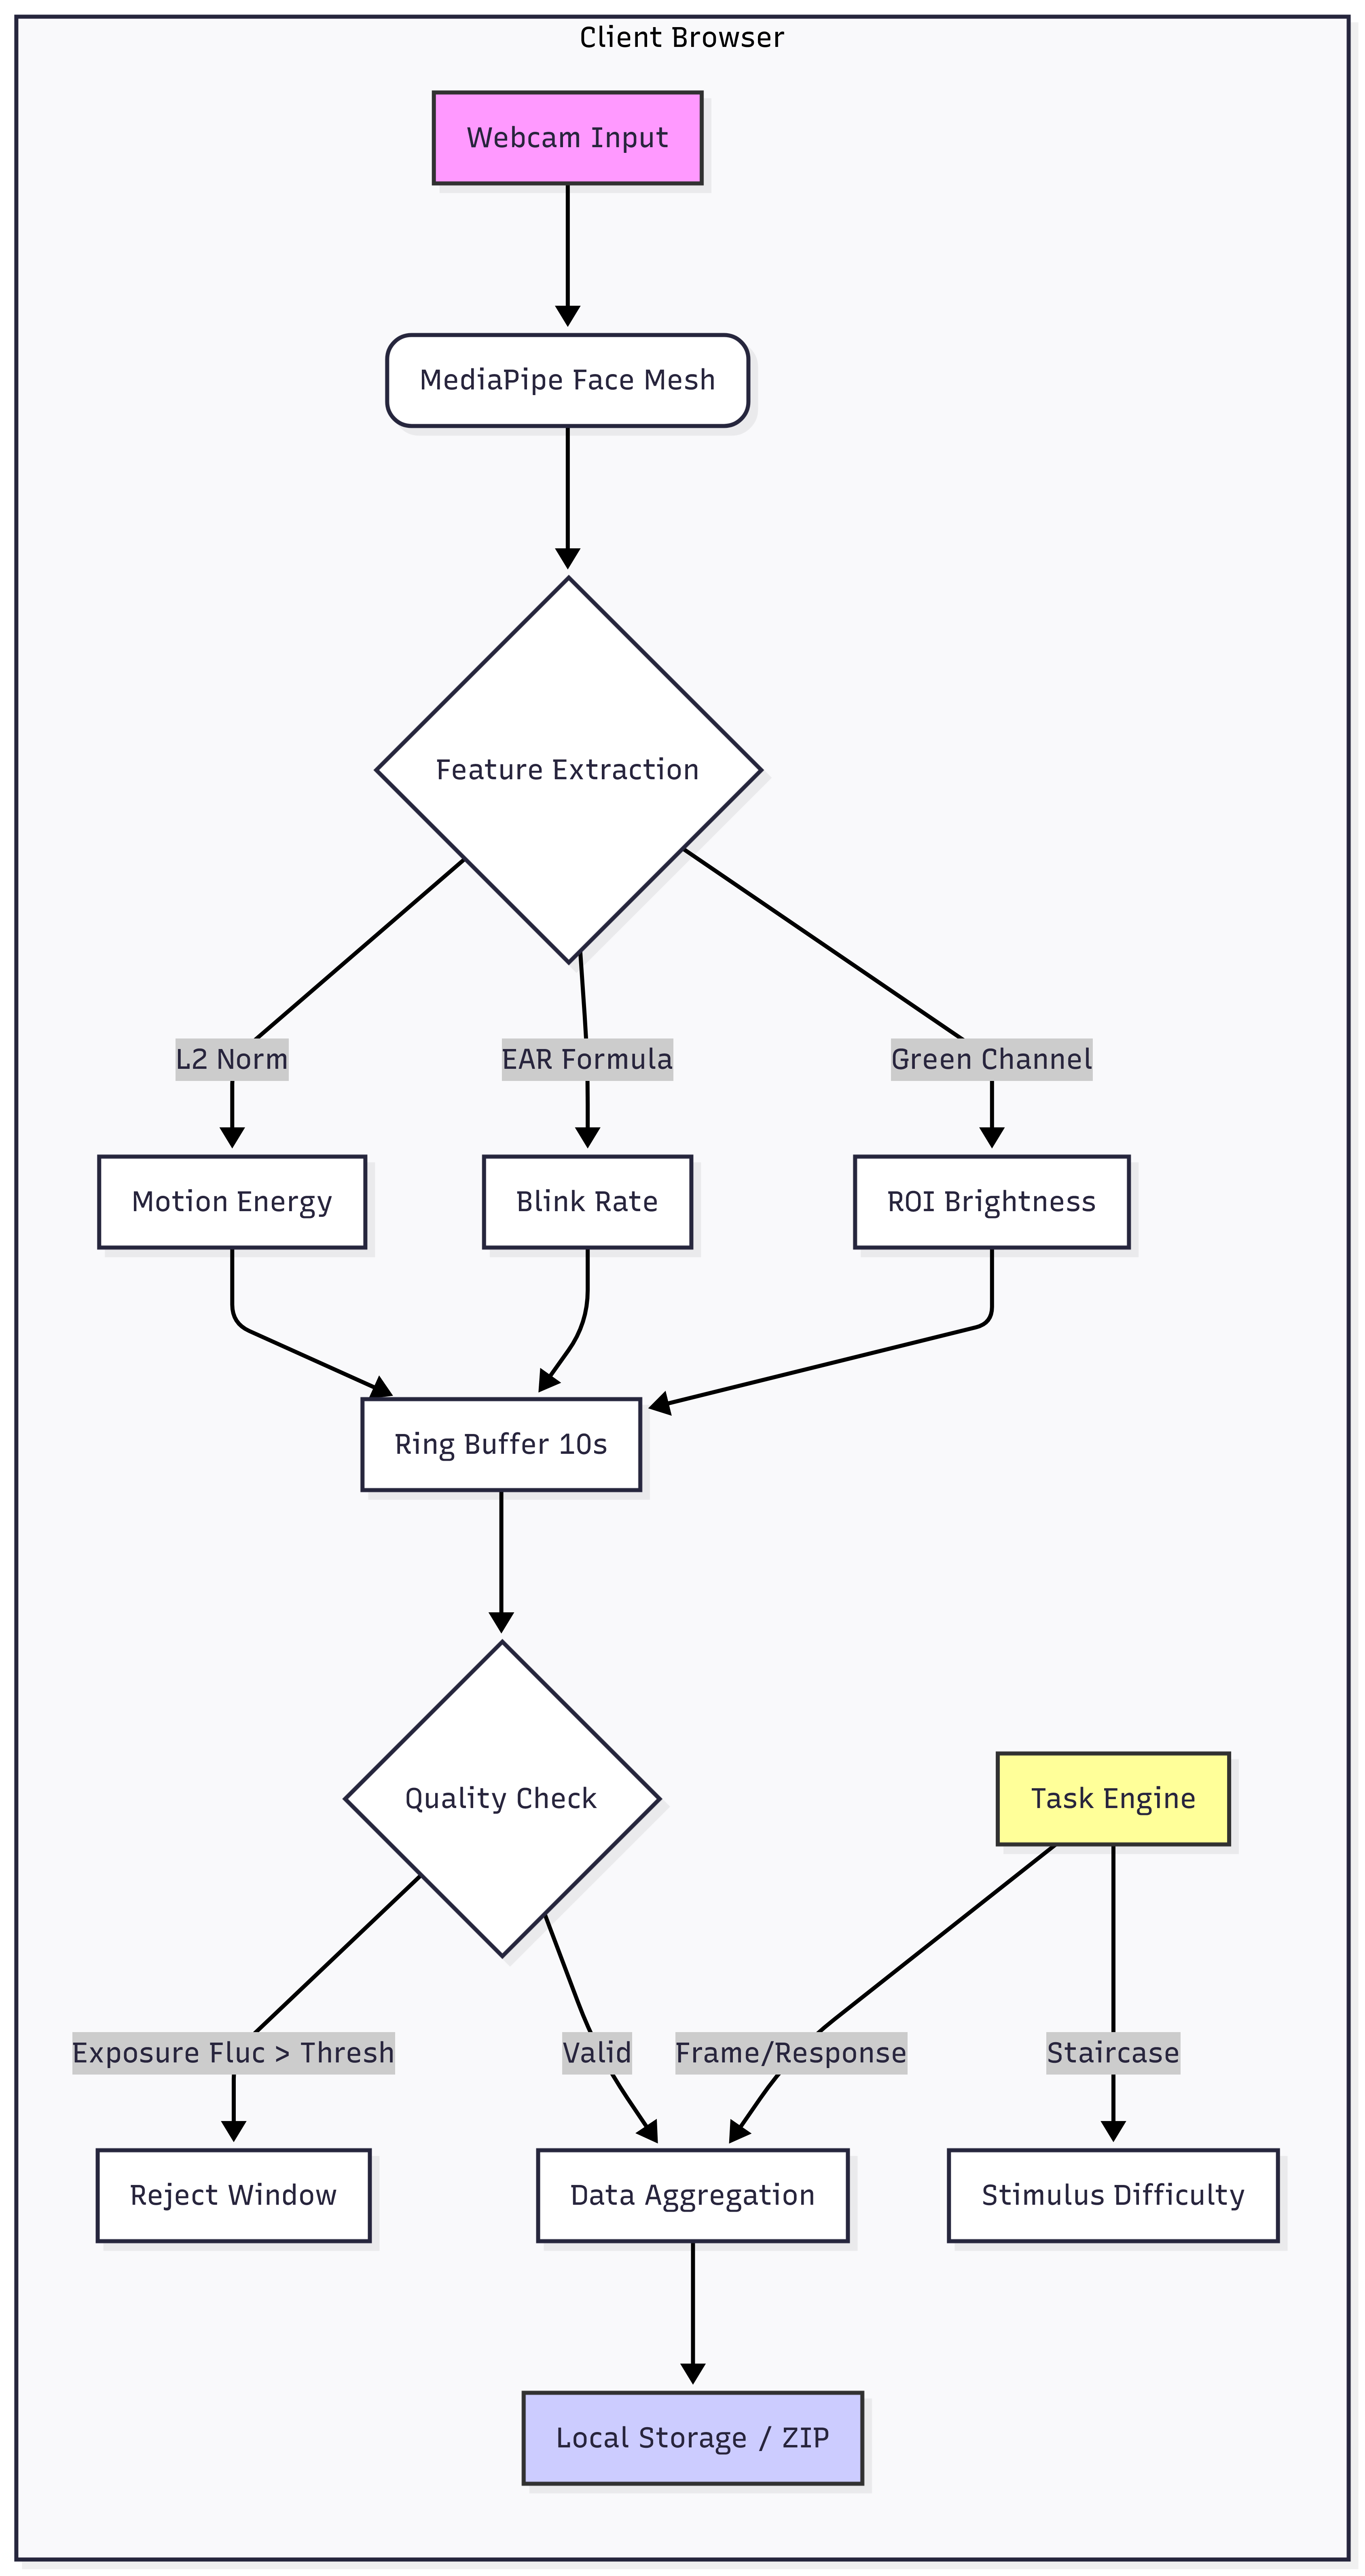
\includegraphics[width=\linewidth]{paper_figures/Figure1_SystemPipeline.png}
%DIFDELCMD <     %%%
\DIFdelendFL \DIFaddbeginFL 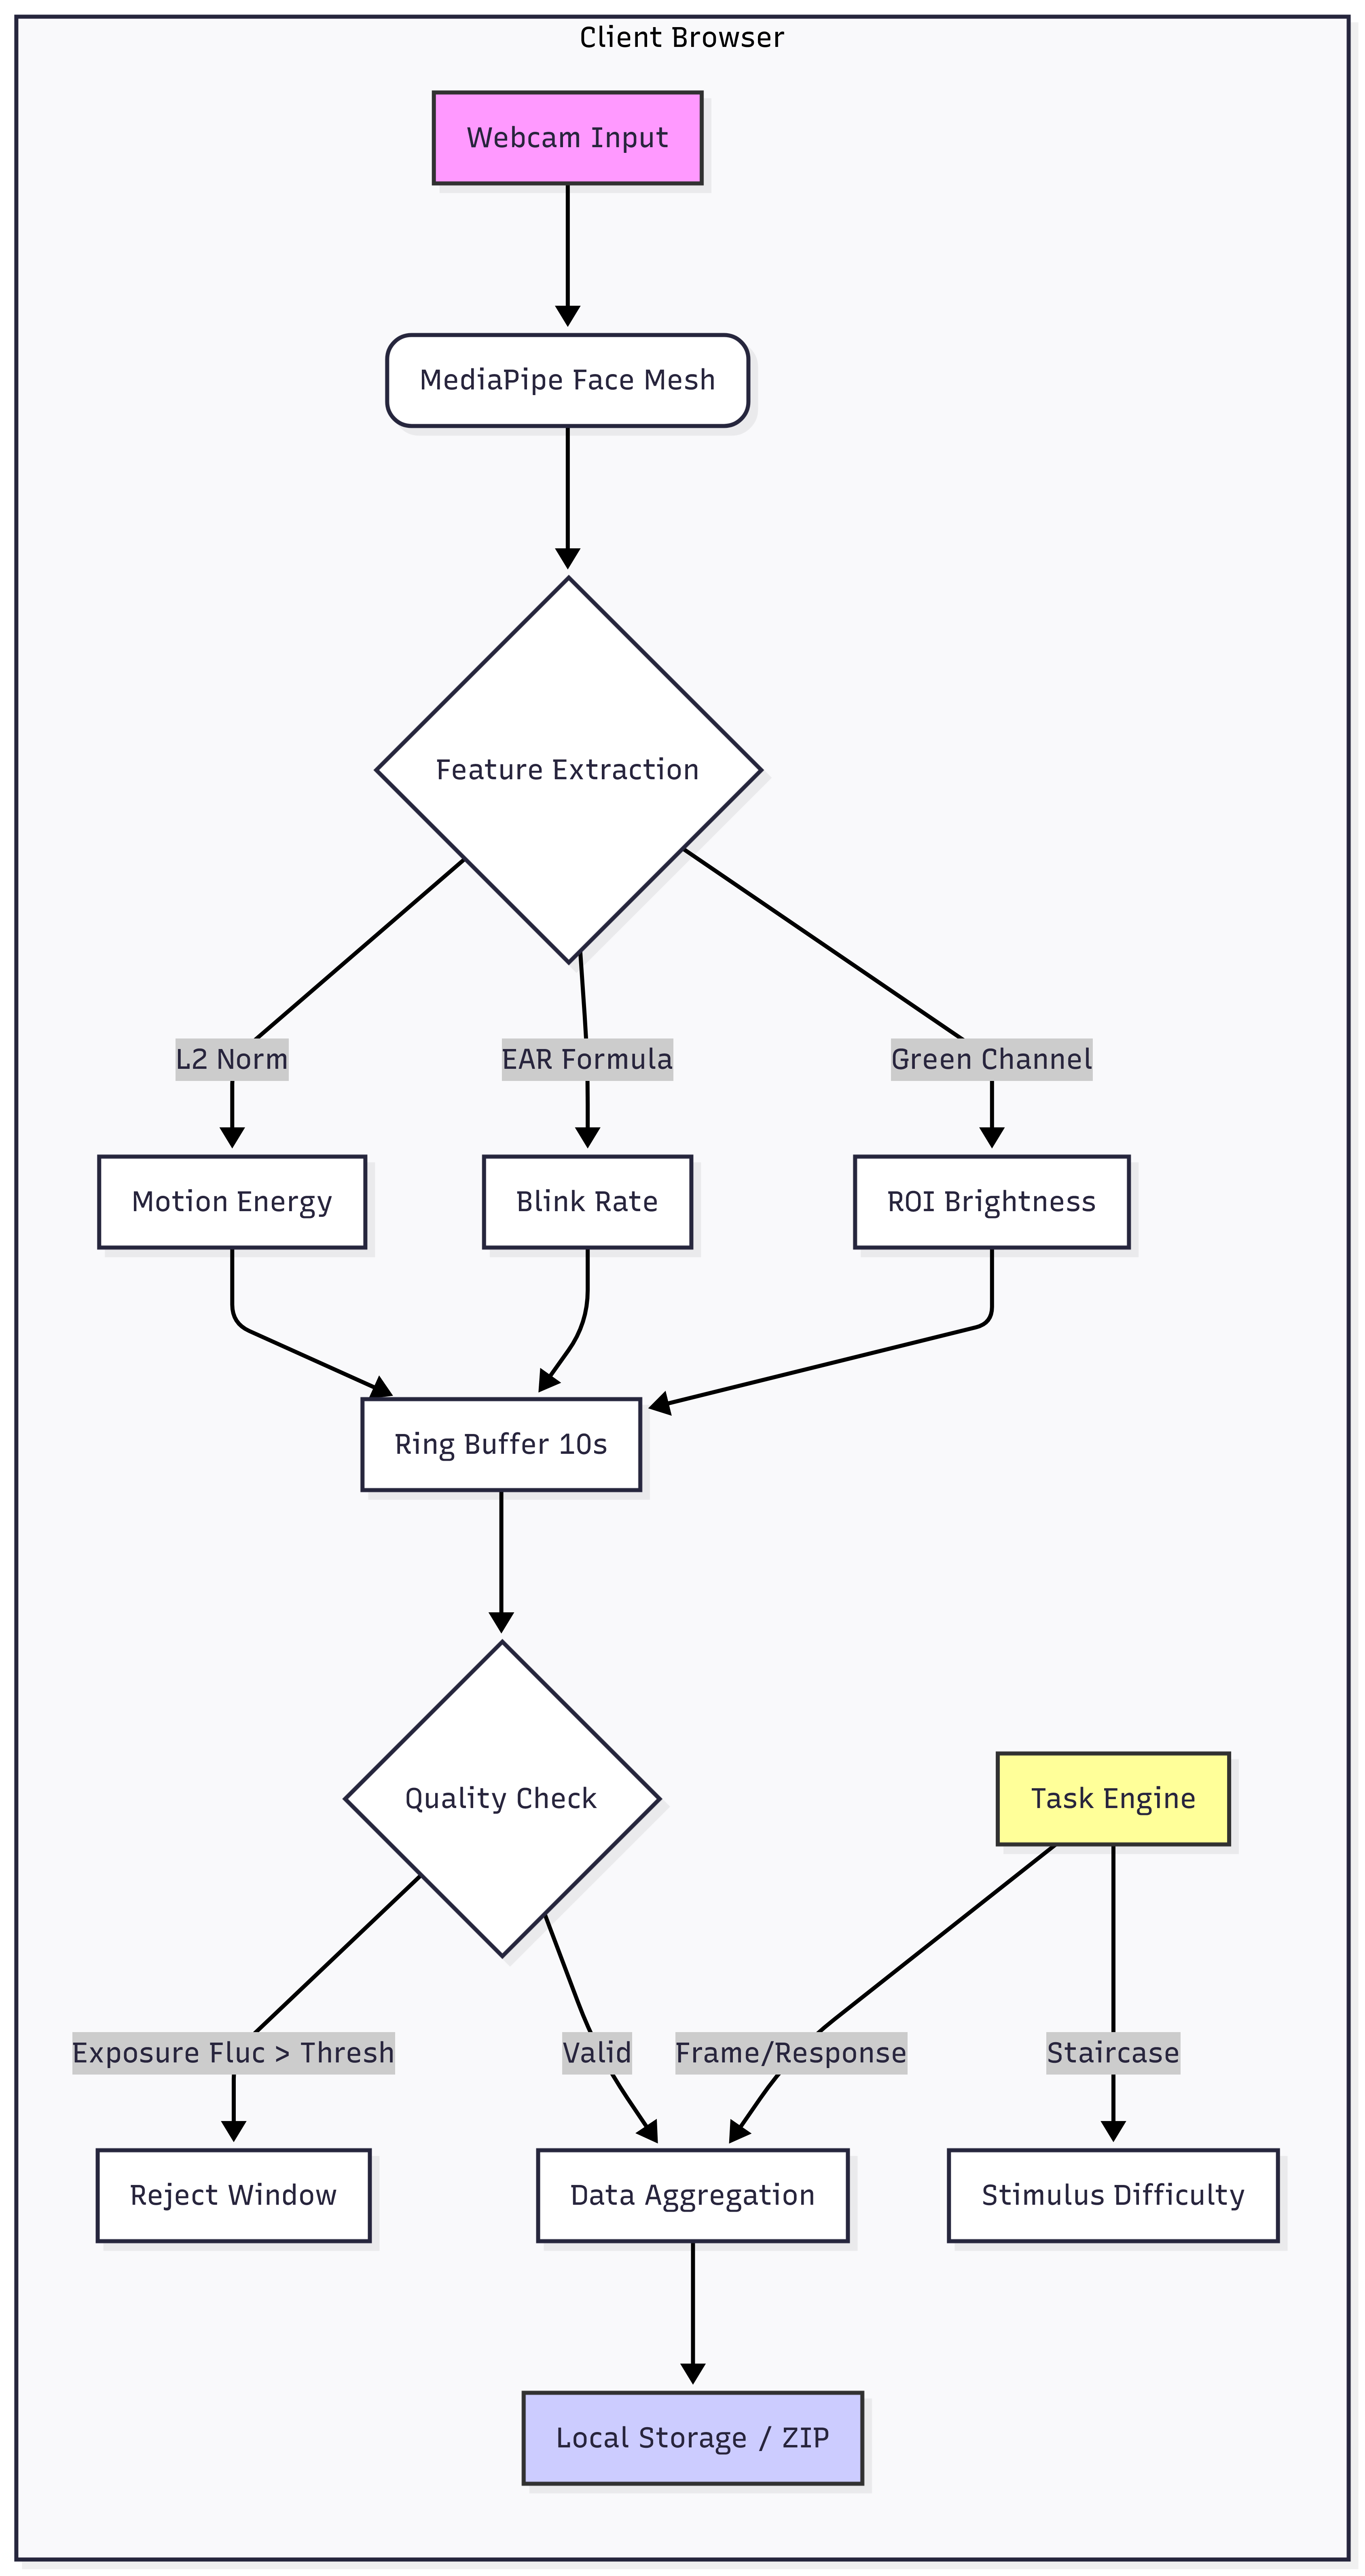
\includegraphics[width=.95\linewidth]{paper_figures/Figure1_SystemPipeline.png}
    \DIFaddendFL \caption{Overview of the Camerala \DIFdelbeginFL \DIFdelFL{System Architecture}\DIFdelendFL \DIFaddbeginFL \DIFaddFL{system architecture}\DIFaddendFL . The \DIFdelbeginFL \DIFdelFL{system runs entirely client-side, processing }\DIFdelendFL \DIFaddbeginFL \DIFaddFL{browser obtains }\DIFaddendFL webcam frames\DIFdelbeginFL \DIFdelFL{via MediaPipe Face Mesh (Wasm) to extract rPPG }\DIFdelendFL \DIFaddbeginFL \DIFaddFL{, extracts FaceMesh/rPPG-oriented features }\DIFaddendFL and \DIFdelbeginFL \DIFdelFL{Head Motion signals in real-time. Data is synchronized }\DIFdelendFL \DIFaddbeginFL \DIFaddFL{quality indicators, synchronizes them }\DIFaddendFL with \DIFdelbeginFL \DIFdelFL{the Psychophysics Task Engine (Canvas API) }\DIFdelendFL \DIFaddbeginFL \DIFaddFL{task events, }\DIFaddendFL and \DIFdelbeginFL \DIFdelFL{stored locally}\DIFdelendFL \DIFaddbeginFL \DIFaddFL{exports local logs. Under the tested implementation}\DIFaddendFL , \DIFdelbeginFL \DIFdelFL{ensuring no }\DIFdelendFL \DIFaddbeginFL \DIFaddFL{only extracted features and task events are logged; }\DIFaddendFL raw video \DIFdelbeginFL \DIFdelFL{ever leaves the user's device}\DIFdelendFL \DIFaddbeginFL \DIFaddFL{is neither transmitted nor stored by Camerala}\DIFaddendFL .}
    \label{fig:system_architecture}
\end{center}
\end{figure}

\subsection{High-Level Architecture}
The system enables a \DIFdelbegin \DIFdel{complete experimental loop entirely within }\DIFdelend \DIFaddbegin \DIFadd{task-constrained experimental loop inside }\DIFaddend the browser sandbox (\DIFdelbegin \DIFdel{see }\DIFdelend Fig. \ref{fig:system_architecture}).
The architecture consists of three coupled modules\DIFdelbegin \DIFdel{running on the main JavaScript thread and dedicated WebWorkers}\DIFdelend :
\begin{enumerate}
    \item \textbf{\DIFdelbegin \DIFdel{The }\DIFdelend Task Engine}: \DIFdelbegin \DIFdel{Responsible for stimulus }\DIFdelend \DIFaddbegin \DIFadd{Stimulus }\DIFaddend rendering, trial logic, \DIFdelbegin \DIFdel{and reaction time measurement}\DIFdelend \DIFaddbegin \DIFadd{key responses, feedback, staircase updates, and reaction-time logging}\DIFaddend .
    \item \textbf{\DIFdelbegin \DIFdel{The }\DIFdelend Vision Pipeline}: \DIFdelbegin \DIFdel{Responsible for ingesting the webcam stream, performing facial landmark inference, and extracting raw physiological signals}\DIFdelend \DIFaddbegin \DIFadd{Webcam ingestion, MediaPipe Face Mesh inference, rPPG-oriented ROI feature extraction, head-motion estimates, blink/EAR features, and frame-level quality indicators}\DIFaddend .
    \item \textbf{\DIFdelbegin \DIFdel{The }\DIFdelend Data Manager}: \DIFdelbegin \DIFdel{Responsible for fusing the asynchronous streams (Vision Frame Time vs. Task Event Time) and securing data persistence }\DIFdelend \DIFaddbegin \DIFadd{Timestamp alignment, trial/frame aggregation, CSV serialization, ZIP packaging, and local persistence without raw-video storage}\DIFaddend .
\end{enumerate}

\subsection{Technical Implementation: The Vision Pipeline}
\DIFdelbegin \DIFdel{We utilize the }\DIFdelend \DIFaddbegin \DIFadd{The current implementation uses }\DIFaddend MediaPipe Face Mesh \DIFdelbegin \DIFdel{\mbox{%DIFAUXCMD
\cite{mediapipe_paper} }\hskip0pt%DIFAUXCMD
solution, which provides 468 3D facial landmarks in real-time.
This model is executed via TensorFlow.js with the WebGL backend to leverage the client's GPU acceleration}\DIFdelend \DIFaddbegin \DIFadd{as a software framework for browser-based facial landmark extraction \mbox{%DIFAUXCMD
\cite{mediapipe_framework}}\hskip0pt%DIFAUXCMD
.
The camera stream is requested through }\texttt{\DIFadd{getUserMedia}} \DIFadd{with ideal constraints of 640$\times$480 pixels and 30 fps.
Because actual camera settings can depend on the browser and device, these constraints should be interpreted as requested settings rather than verified hardware settings}\DIFaddend .

\subsubsection{Feature Extraction Logic}
\DIFdelbegin \DIFdel{To quantify behaviorally relevant and motion-related features , we extract two primary signals: }\textit{\DIFdel{Head Motion Index}} %DIFAUXCMD
\DIFdel{and }\textit{\DIFdel{Exposure Fluctuation}}%DIFAUXCMD
\DIFdel{.
}\DIFdelend \DIFaddbegin \DIFadd{The present implementation records sensor-derived features and quality indicators rather than validated clinical or medical measurements.
Two categories are central to this paper:
}\DIFaddend 

\textbf{1. Head Motion Index ($M_t$)}
\DIFdelbegin \DIFdel{To estimate participant stability and gross motor movement, we track the displacement of rigid cranial landmarks (Nose tip, Left/Right Tragus) that are generally unaffected by facial expressions.
Let $L_i^t = (x_i^t, y_i^t, z_i^t)$ be the 3D coordinate of the $i$-th landmark }\DIFdelend \DIFaddbegin \DIFadd{Head motion is approximated from the frame-to-frame displacement of a facial landmark.
Let $L^t = (x^t, y^t)$ be the normalized landmark coordinate }\DIFaddend at frame $t$.
The \DIFdelbegin \DIFdel{instantaneous motion scalar $M_t$ is defined asthe Euclidean distance summed over the set of rigid landmarks $S_{rigid} = \{1, 33, 263\}$ (Nose, L-Ear, R-Ear):
}\DIFdelend \DIFaddbegin \DIFadd{motion scalar is computed as:
}\DIFaddend \begin{equation}
    M_t = \DIFdelbegin \DIFdel{\frac{1}{|S_{rigid}|} \sum_{i \in S_{rigid}} }\DIFdelend || L\DIFdelbegin \DIFdel{_i}\DIFdelend ^t - L\DIFdelbegin \DIFdel{_i}\DIFdelend ^{t-1} ||_2 \DIFaddbegin \DIFadd{.
}\DIFaddend \end{equation}
\DIFdelbegin \DIFdel{To ensure scale invariance (handling users sitting at different distances), the coordinates are normalized by the Inter-Ocular Distance (IOD),
calculated as the Euclidean distance between the lateral canthi of the eyes.
}\DIFdelend \DIFaddbegin \DIFadd{This feature is used as a motion-related quality and behavior indicator.
It is not an algorithmic correction for motion artifacts in rPPG.
}\DIFaddend 

\DIFdelbegin \textbf{\DIFdel{2. Exposure Fluctuation ($E_{fluc}$)}}
%DIFAUXCMD
\DIFdel{Deploying sensors outside the lab introduces variable lighting.
In a home environment, clouds passing the sun, screens flickering, or power cycles induce luminance changes that can mask the rPPG signal.
We quantify this frame-level luminance fluctuation as an environmental quality indicator.
We define a Region of Interest (ROI ) on the forehead, $R_{fore}$.
The average luminance $Y_t$ is computed from the RGB channels:
}\DIFdelend \DIFaddbegin \textbf{\DIFadd{2. ROI Green-Channel Value and Brightness-Change Indicator}}
\DIFadd{The implementation samples a small forehead region around a FaceMesh landmark and records the green-channel brightness as an rPPG-oriented ROI value.
It also computes a frame-to-frame green-channel brightness-change indicator:
}\DIFaddend \begin{equation}
    \DIFaddbegin \DIFadd{B_{\Delta}(t) = | G_t - G_{t-1} | ,
}\DIFaddend \end{equation}
\DIFdelbegin \DIFdel{The Exposure Fluctuation metric is then defined as the first derivative of luminance:
}\begin{displaymath}
    \DIFdel{E_{fluc}(t) = | Y_t - Y_{t-1} |
}\end{displaymath}%DIFAUXCMD
\DIFdelend \DIFaddbegin \DIFadd{where $G_t$ is the downsampled frame-level green-channel average at frame $t$.
Camerala does not attempt to correct rPPG degradation caused by motion or illumination changes.
Instead, it records motion-related and brightness-related indicators for descriptive inspection of exported records.
The brightness-change indicator does not measure camera exposure settings, external illuminance, specific environmental events, psychological or physiological state, or rPPG accuracy.
}\DIFaddend 

\subsection{Technical Implementation: The Task Engine}
The experimental psychophysical probe is a \DIFdelbegin \textbf{\DIFdel{2-Alternative Forced Choice (2AFC) Orientation Discrimination Task}}%DIFAUXCMD
\DIFdel{.
}%DIFDELCMD < 

%DIFDELCMD < %%%
\subsubsection{\DIFdel{Stimulus Generation via Canvas API}}
%DIFAUXCMD
\addtocounter{subsubsection}{-1}%DIFAUXCMD
\DIFdelend \DIFaddbegin \DIFadd{two-alternative forced-choice orientation discrimination task.
}\DIFaddend Using the HTML5 Canvas API, \DIFdelbegin \DIFdel{we procedurally generate Gabor patches. A Gabor patch is defined as a sinusoidal grating multiplied by a Gaussian envelope.
The luminance profile $L(x,y)$ is given by:
}\begin{displaymath}
    \DIFdel{L(x,y) = L_0 + C \cdot \exp\left(-\frac{x'^2 + \gamma^2 y'^2}{2\sigma^2}\right) \cdot \cos\left(2\pi \frac{x'}{\lambda} + \phi\right)
}\end{displaymath}%DIFAUXCMD
\DIFdel{Where:
}%DIFDELCMD < \begin{itemize}
%DIFDELCMD <     \item %%%
\DIFdel{$L_0$: Background luminance (128/255 gray).
    }%DIFDELCMD < \item %%%
\DIFdel{$C$: Contrast of the grating.
    }%DIFDELCMD < \item %%%
\DIFdel{$\lambda$: Wavelength (spatial frequency).
    }%DIFDELCMD < \item %%%
\DIFdel{$\theta$: Orientation angle (the target variable: $+45^\circ$ or $-45^\circ$).
    }%DIFDELCMD < \item %%%
\DIFdel{$x', y'$: Coordinates rotated by $\theta$}\DIFdelend \DIFaddbegin \DIFadd{the task engine procedurally renders oriented grating stimuli, records key responses, calculates reaction time with }\texttt{\DIFadd{performance.now()}}\DIFadd{, and updates task difficulty.
Procedural rendering avoids network-dependent stimulus loading during a trial and keeps task timing in the same browser runtime as feature logging}\DIFaddend .
\DIFdelbegin %DIFDELCMD < \end{itemize}
%DIFDELCMD < %%%
\DIFdel{By generating stimuliprocedurally rather than loading image files, we eliminate network latency and ensure pixel-perfect control
over the spatial frequency and contrast.
}\DIFdelend 

\subsubsection{Timing and Synchronization}
\DIFdelbegin \DIFdel{Web-based reaction time measurement is notoriously jittery. To mitigate this, we employ}\DIFdelend \DIFaddbegin \DIFadd{The implementation uses the following timing strategy}\DIFaddend :
\begin{enumerate}
    \item \textbf{\DIFdelbegin \DIFdel{High-Res Time}\DIFdelend \DIFaddbegin \DIFadd{High-resolution timestamps}\DIFaddend }: \DIFdelbegin \DIFdel{All timestamps use }\DIFdelend \DIFaddbegin \DIFadd{Task events and frame features are timestamped using }\DIFaddend \texttt{performance.now()}\DIFdelbegin \DIFdel{, which provides high-resolution timestamps independent of the system clock}\DIFdelend .
    \item \textbf{\DIFdelbegin \DIFdel{Frame-Locked Rendering}\DIFdelend \DIFaddbegin \DIFadd{Frame-loop alignment}\DIFaddend }: \DIFdelbegin \DIFdel{Stimulus rendering is synchronized using }\texttt{\DIFdel{requestAnimationFrame}}%DIFAUXCMD
\DIFdel{.
    We log the timestamp of the frame }\textit{\DIFdel{immediately}} %DIFAUXCMD
\DIFdel{before the stimulus paint command}\DIFdelend \DIFaddbegin \DIFadd{Feature extraction and task rendering are coordinated with the browser frame loop}\DIFaddend .
    \item \textbf{\DIFdelbegin \DIFdel{Low-Latency Sync}\DIFdelend \DIFaddbegin \DIFadd{Local runtime alignment}\DIFaddend }: \DIFdelbegin \DIFdel{On-device processing avoids network transmission during task-aligned sensing and keeps task and sensing timestamps within the same local runtimein the present design}\DIFdelend \DIFaddbegin \DIFadd{Task events and sensor-derived features are logged in the same browser runtime, avoiding server-side reconciliation}\DIFaddend .
\end{enumerate}

\begin{algorithm}
\caption{Camerala Task Loop (Simplified)}
\begin{algorithmic}
\STATE \textbf{Initialize} Camera, FaceMesh, Canvas
\DIFaddbegin \STATE \DIFadd{StartContinuousVisionFrameLoop()
}\DIFaddend \WHILE{Session Active}
    \STATE $Block \leftarrow$ GetCurrentBlock()
    \STATE \DIFdelbegin \DIFdel{$Condition \leftarrow Block.condition$
    }\DIFdelend \DIFaddbegin \DIFadd{$Context \leftarrow Block.instruction$
    }\DIFaddend \STATE ShowInstruction(\DIFdelbegin \DIFdel{Condition}\DIFdelend \DIFaddbegin \DIFadd{Context}\DIFaddend .text)
    \DIFdelbegin %DIFDELCMD < \FOR{trial $i = 1$ to 20}
%DIFDELCMD <         %%%
\DIFdelend \DIFaddbegin \FOR{trial $i = 1$ to $n$}
        \DIFaddend \STATE \DIFdelbegin \textbf{\DIFdel{Fixation Phase}}%DIFAUXCMD
\DIFdel{: Show Cross ($500ms + \mathcal{U}(0, 200)ms$}\DIFdelend \DIFaddbegin \DIFadd{$\theta \leftarrow$ SampleOrientation(\{-45$^\circ$, +45$^\circ$\}}\DIFaddend )
        \STATE \DIFaddbegin \DIFadd{ShowFixation(400--600 ms)
        }\STATE \DIFaddend $t_{onset} \leftarrow$ performance.now()
        \STATE \DIFdelbegin \DIFdel{DrawGaborPatch($\theta_i$}\DIFdelend \DIFaddbegin \DIFadd{DrawOrientationStimulus($\theta$, 200 ms}\DIFaddend )
        \WHILE{No KeyPress}
            \STATE Poll \DIFdelbegin \DIFdel{Keyboard Input
        }\DIFdelend \DIFaddbegin \DIFadd{F/J KeyPress
        }\DIFaddend \ENDWHILE
        \STATE $t_{response} \leftarrow$ performance.now()
        \STATE $RT \leftarrow t_{response} - t_{onset}$
        \STATE \DIFdelbegin \DIFdel{$Accuracy \leftarrow (Key == Target)$
        }%DIFDELCMD < \STATE %%%
\textbf{\DIFdel{Feedback}}%DIFAUXCMD
\DIFdel{: Show Color (Green/Red}\DIFdelend \DIFaddbegin \DIFadd{LogTaskEvent($RT$, Accuracy, Context}\DIFaddend )
        \STATE UpdateStaircase(Accuracy\DIFaddbegin \DIFadd{, relative $\pm$5\% contrast step}\DIFaddend )
        \STATE \DIFdelbegin \DIFdel{$Log(RT, Accuracy, FaceMeshFeatures)$
    }\DIFdelend \DIFaddbegin \DIFadd{LinkTaskEventToFrameTimestamps($t_{onset}$, $t_{response}$, Context)
    }\DIFaddend \ENDFOR
\ENDWHILE
\end{algorithmic}
\end{algorithm}

\subsection{Data Management and \DIFdelbegin \DIFdel{Privacy}\DIFdelend \DIFaddbegin \DIFadd{Local-First Persistence}\DIFaddend }
\DIFdelbegin \DIFdel{Since no server is involved, data persistence is handled via the }\textbf{\DIFdel{File System Access API}} %DIFAUXCMD
\DIFdel{(on supported browsers) or a fallback to }\texttt{\DIFdel{Blob}} %DIFAUXCMD
\DIFdel{download.
Data is serialized into JSON Lines (.jsonl) format. Each line represents one frame or one trial event. This allows for streaming writes, ensuring that even if the browser crashes mid-session, data up to that point is preserved.
At the end of a session}\DIFdelend \DIFaddbegin \DIFadd{The current implementation uses JSZip to export local log files as a ZIP archive.
The archive contains }\texttt{\DIFadd{metadata.json}}\DIFadd{, }\texttt{\DIFadd{trials.csv}}\DIFaddend , \DIFdelbegin \DIFdel{the user initiates a "Download Data" action, which zips the JSON logs and saves them to their local disk.
This explicit user action reinforces the sense of agency and privacy control.
}\DIFdelend \DIFaddbegin \texttt{\DIFadd{features\_raw.csv}}\DIFadd{, }\texttt{\DIFadd{windows.csv}}\DIFadd{, }\texttt{\DIFadd{blocks.csv}}\DIFadd{, and }\texttt{\DIFadd{subjective.csv}}\DIFadd{.
The metadata file stores the session ID, start time, user agent, and block plan.
The user initiates the download at the end of the session.
This design avoids Camerala-side raw-video storage and avoids raw-video transmission, but it also reduces the ability to inspect image artifacts retrospectively.
For this reason, Camerala logs reproducible exported fields such as rPPG-oriented ROI green-channel values, head-motion estimates, and a frame-to-frame green-channel brightness-change indicator.
}\DIFaddend 

%DIF >  =================================================================================
%DIF >  SECTION 4: METHODOLOGY
%DIF >  =================================================================================
\section{Methodology}

\DIFdelbegin \subsection{\DIFdel{Longitudinal Exploratory Deployment}}
%DIFAUXCMD
\addtocounter{subsection}{-1}%DIFAUXCMD
\DIFdel{To evaluate the operational deployability of Camerala across different physical environments}\DIFdelend \DIFaddbegin \subsection{\DIFadd{Target Usage Scenario and Exploratory Deployment}}
\DIFadd{The target use case is a remote psychological or psychophysiological task experiment conducted while the participant is seated in front of a laptop.
It is not intended to represent continuous sensing during ordinary daily activities such as walking, cooking, conversation, or sleep.
The tested deployment therefore concerns a task-constrained experiment conducted in laboratory and home settings, with browser-based logging of behavioral events and webcam-derived features.
}

\DIFadd{To evaluate operational completion under this scenario}\DIFaddend , we conducted an exploratory longitudinal deployment \DIFdelbegin \DIFdel{(N=1).
While traditional between-subjects group designs (Large-N) are strictly necessary for estimating generalizable psychological effects, an intensive N=1 autoethnography (Trials=}\DIFdelend \DIFaddbegin \DIFadd{with one author-participant.
The deployment consisted of 10 sessions and }\DIFaddend 600 \DIFdelbegin \DIFdel{) serves as a technical proof-of-concept for the }\textit{\DIFdel{system architecture}}%DIFAUXCMD
\DIFdel{.
This design allows us to observe the system's operational continuity across contrasting ecological conditions without the compounding variance of diverse user demographics.
The study followed an A-B-C logic within each session (see Fig. 4), varying the explicit instructional framing conditions presented to the user (Neutral, Negative Evaluation, Positive Evaluation).
Each session consisted of 3 Blocks (60 trials total), order-balanced via a Latin Square design to prevent order effects}\DIFdelend \DIFaddbegin \DIFadd{total trials.
Each session consisted of six 10-trial blocks, with two blocks for each instructional task context (neutral instruction, negative instruction, and positive instruction), as reflected in the exported block plans.
The order of blocks was randomized by the web application}\DIFaddend .

\DIFdelbegin %DIFDELCMD < \begin{figure}[t]
%DIFDELCMD <     \begin{center}
%DIFDELCMD <     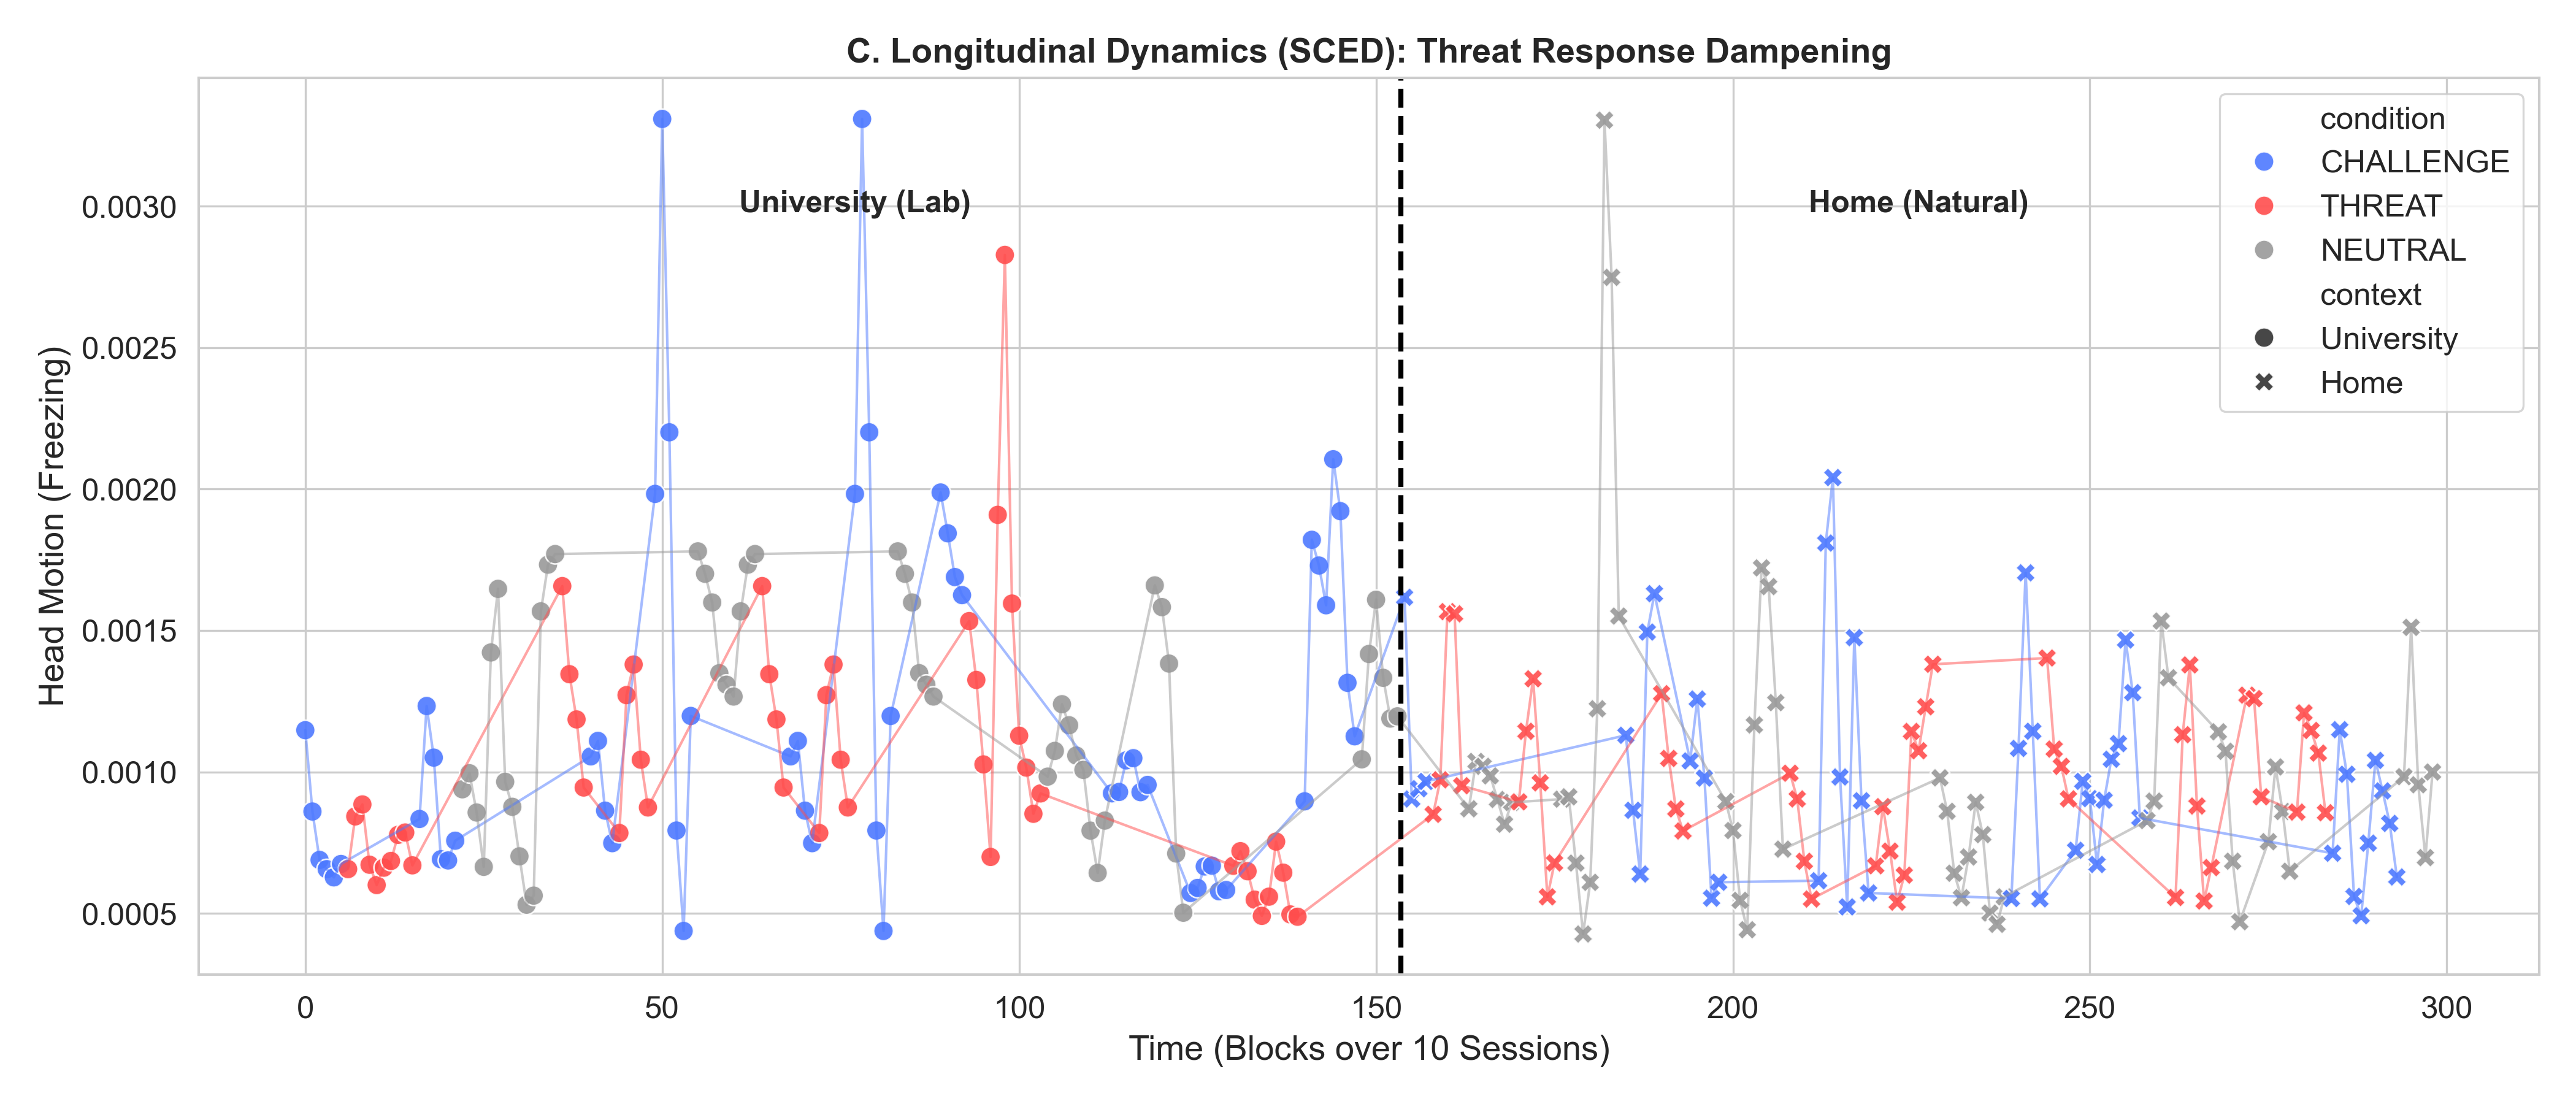
\includegraphics[width=\linewidth]{paper_figures/Figure4_Longitudinal.png}
%DIFDELCMD <     %%%
%DIFDELCMD < \caption{%
{%DIFAUXCMD
\DIFdelFL{Visual representation of the deployment schedule. The study spanned 14 days, alternating between Home and Lab environments. Each session consisted of 3 blocks with randomized order, totaling 600 trials. This approach allows for robust observation of between-environment signal differences.}}
    %DIFAUXCMD
%DIFDELCMD < \label{fig:sced_design}
%DIFDELCMD < \end{center}
%DIFDELCMD < \end{figure}
%DIFDELCMD < 

%DIFDELCMD < %%%
\DIFdelend \subsection{Participant (Autoethnography)}
\DIFdelbegin \DIFdel{In line with standard systems feasibility evaluation, the }\DIFdelend \DIFaddbegin \DIFadd{The }\DIFaddend participant was the primary author.
\DIFdelbegin \textit{\DIFdel{Ethical Note}}%DIFAUXCMD
\DIFdel{: }\DIFdelend This was a self-experimentation \DIFdelbegin \DIFdel{(autoethnographic) evaluation. No }\DIFdelend \DIFaddbegin \DIFadd{evaluation: no }\DIFaddend other participants were involved, no identifiable \DIFaddbegin \DIFadd{raw }\DIFaddend video was transmitted \DIFdelbegin \DIFdel{or shared}\DIFdelend \DIFaddbegin \DIFadd{by Camerala}\DIFaddend , and the author provided informed consent for self-participation.
\DIFdelbegin \DIFdel{We explicitly acknowledge that the author's prior knowledge of the experimental hypotheses precludes drawing population-level psychological conclusions.
However, this deploymentis methodologically appropriate for the initial technical validation of the sensing pipeline.
}\DIFdelend \DIFaddbegin \DIFadd{Because the participant was also the author and knew that the task instructions were experimental, the instruction blocks cannot be assumed to have induced evaluation pressure, reward motivation, or psychological effects.
They are used only as different instructional task contexts for demonstrating synchronized logging across task conditions.
}\DIFaddend 

\DIFaddbegin \subsection{\DIFadd{Hardware and Software Configuration}}
\DIFadd{Table \ref{tab:hardware_config} reports the hardware/software configuration used in the deployment.
}

\begin{table*}[t]
\caption{\DIFaddFL{Hardware and software configuration}}
\label{tab:hardware_config}
\begin{center}
\small
\begin{tabular}{p{0.28\textwidth}p{0.64\textwidth}}
\toprule
\textbf{\DIFaddFL{Item}} & \textbf{\DIFaddFL{Reported value}} \\
\midrule
\DIFaddFL{Laptop/PC model }& \DIFaddFL{mouse Computer G-Tune P517G60ZO21CNHWT, 15.6-inch gaming notebook }\\
\DIFaddFL{CPU }& \DIFaddFL{Intel Core i7-13620H }\\
\DIFaddFL{GPU }& \DIFaddFL{NVIDIA GeForce RTX 5060 Laptop GPU }\\
\DIFaddFL{RAM }& \DIFaddFL{32 GB }\\
\DIFaddFL{Storage }& \DIFaddFL{1 TB SSD }\\
\DIFaddFL{Operating system }& \DIFaddFL{Windows 11 Home 64-bit }\\
\DIFaddFL{Browsers used }& \DIFaddFL{Mozilla Firefox and Google Chrome }\\
\DIFaddFL{Recorded browser metadata }& \DIFaddFL{Session metadata stored browser user-agent strings. Mozilla Firefox and Google Chrome were used in the deployment, but browser effects were not independently manipulated or analyzed. }\\
\DIFaddFL{Webcam type/model }& \DIFaddFL{Built-in laptop webcam }\\
\DIFaddFL{Requested camera constraints }& \texttt{\DIFaddFL{getUserMedia}}\DIFaddFL{: ideal 640$\times$480 pixels, ideal 30 fps }\\
\DIFaddFL{Camera capture behavior }& \DIFaddFL{Browser-negotiated capture under the requested constraints; no manual exposure or white-balance constraints were applied }\\
\DIFaddFL{Processing rate }& \DIFaddFL{Not analyzed as a result metric in the present revision }\\
\DIFaddFL{Display }& \DIFaddFL{Built-in 15.6-inch display, 2560$\times$1440 pixels, 165 Hz }\\
\DIFaddFL{Screen brightness }& \DIFaddFL{Fixed across sessions using the built-in laptop display setting }\\
\DIFaddFL{Viewing distance }& \DIFaddFL{Approximately 50--60 cm }\\
\DIFaddFL{Auto-exposure }& \DIFaddFL{Device/browser default camera pipeline; no manual exposure control was applied }\\
\DIFaddFL{Auto-white-balance }& \DIFaddFL{Device/browser default camera pipeline; no manual white-balance control was applied }\\
\bottomrule
\end{tabular}
\end{center}
\end{table*}

\DIFaddend \subsection{\DIFdelbegin \DIFdel{Apparatus and Physical }\DIFdelend \DIFaddbegin \DIFadd{Deployment }\DIFaddend Environment \DIFaddbegin \DIFadd{and Lighting Conditions}\DIFaddend }
The \DIFdelbegin \DIFdel{experiment was deployed on a standard 13.5-inch laptop display (approximate 60Hz target refresh rate).
To contextualize the environmental differences, ambient illuminance was estimated using a digital lux meter at the eye level of the participant.
}%DIFDELCMD < \begin{itemize}
%DIFDELCMD <     \item %%%
\textbf{\DIFdel{Lab Environment}}%DIFAUXCMD
\DIFdel{: Mean illuminance $480 \pm 20$ lux (Standard fluorescent lighting ).
}%DIFDELCMD < \item %%%
\DIFdelend \DIFaddbegin \DIFadd{deployment was conducted during daytime in an indoor university laboratory/research room and an indoor private home room under general artificial room lighting.
Both rooms had windows, but curtains were closed during the sessions.
Direct natural light was not used as the primary illumination source in either context.
The built-in laptop display brightness was fixed across sessions.
Because the deployment used camera-derived setup checks rather than external light-meter measurements, this paper reports brightness ranges only as author-confirmed setup/check information.
The camera-derived brightness range observed during setup/checks was 105--114 in the laboratory setting and 102--111 in the home setting.
Table \ref{tab:environment_config} summarizes the deployment environment and lighting conditions.
}

\begin{table*}[t]
\caption{\DIFaddFL{Deployment environment and lighting conditions}}
\label{tab:environment_config}
\begin{center}
\small
\begin{tabular}{p{0.24\textwidth}p{0.32\textwidth}p{0.32\textwidth}}
\toprule
\textbf{\DIFaddFL{Item}} & \textbf{\DIFaddFL{Laboratory}} & \DIFaddendFL \textbf{Home\DIFdelbeginFL \DIFdelFL{Environment}\DIFdelendFL } \DIFdelbeginFL \DIFdelFL{: Mean illuminance $140 \pm 50$ lux (Mixed LED and variable monitor glow).
}%DIFDELCMD < \end{itemize}
%DIFDELCMD < %%%
\DIFdelFL{Distance from the screen was approximately maintained at 50--60 cm, using the FaceMesh tracking standard distance as a rough proxy.
}\DIFdelendFL \DIFaddbeginFL \\
\midrule
\DIFaddFL{Room type }& \DIFaddFL{Indoor university laboratory/research room }& \DIFaddFL{Indoor private home room }\\
\DIFaddFL{Time of day }& \DIFaddFL{Daytime }& \DIFaddFL{Daytime }\\
\DIFaddFL{Primary lighting }& \DIFaddFL{General indoor artificial lighting }& \DIFaddFL{General indoor artificial lighting }\\
\DIFaddFL{Window presence }& \DIFaddFL{Windows present }& \DIFaddFL{Windows present }\\
\DIFaddFL{Curtain/blind condition }& \DIFaddFL{Curtains present and closed }& \DIFaddFL{Curtains present and closed }\\
\DIFaddFL{Natural light contribution }& \DIFaddFL{Direct natural light was not used as the primary illumination source }& \DIFaddFL{Direct natural light was not used as the primary illumination source }\\
\DIFaddFL{Camera-derived brightness range observed during setup/checks }& \DIFaddFL{105--114 }& \DIFaddFL{102--111 }\\
\DIFaddFL{External light-meter measurement }& \multicolumn{2}{p{0.64\textwidth}}{\DIFaddFL{External light-meter values were not used; the reported ranges are camera-derived setup/check information, not lux measurements.}} \\
\DIFaddFL{Screen brightness }& \multicolumn{2}{p{0.64\textwidth}}{\DIFaddFL{Fixed across sessions using the built-in laptop display setting.}} \\
\DIFaddFL{Task display }& \multicolumn{2}{p{0.64\textwidth}}{\DIFaddFL{Stimuli were presented on the built-in laptop display. Screen luminance was part of the tested configuration rather than an independently manipulated factor.}} \\
\DIFaddFL{Window aggregation }& \multicolumn{2}{p{0.64\textwidth}}{\DIFaddFL{Exported window-level features used 10-s windows with 5-s overlap.}} \\
\DIFaddFL{Brightness-change indicator aggregation }& \multicolumn{2}{p{0.64\textwidth}}{\DIFaddFL{The frame-to-frame green-channel brightness-change indicator was summarized in 10-s windows with 5-s overlap.}} \\
\DIFaddFL{Clouds/screen flicker/power cycles }& \multicolumn{2}{p{0.64\textwidth}}{\DIFaddFL{Not treated as observed experimental events; possible brightness variation was handled only as camera-image-derived record variation.}} \\
\bottomrule
\end{tabular}
\end{center}
\end{table*}
\DIFaddend 

\subsection{Experimental Procedure \DIFdelbegin \DIFdel{\& Cognitive Framing}\DIFdelend \DIFaddbegin \DIFadd{and Instructional Task Contexts}\DIFaddend }
Each session began with \DIFdelbegin \DIFdel{an automated }\DIFdelend \DIFaddbegin \DIFadd{a }\DIFaddend pre-session \DIFdelbegin \DIFdel{check used to screen basic capture }\DIFdelend \DIFaddbegin \DIFadd{capture check for basic camera }\DIFaddend conditions, including \DIFdelbegin \DIFdel{luminance, pose, and face size prior to hiding }\DIFdelend \DIFaddbegin \DIFadd{approximate camera-derived brightness and pose, before }\DIFaddend the camera feed \DIFdelbegin \DIFdel{to prevent distraction.
We then presented distinct instructional framing conditions (Neutral, Negative Evaluation, Positive Evaluation) via full-screen text before each 20-trial block.
The }\textbf{\DIFdel{Neutral}} %DIFAUXCMD
\DIFdel{condition served as a baseline.
The }\textbf{\DIFdel{Negative Evaluation}} %DIFAUXCMD
\DIFdel{condition ("WARNING: CRITICAL. Poor performance is unacceptable") served as a negative task framing manipulation.
The }\textbf{\DIFdel{Positive Evaluation}} %DIFAUXCMD
\DIFdel{condition ("BONUS. Break your record!") served as a positive task framing manipulation.
}\DIFdelend \DIFaddbegin \DIFadd{was hidden to reduce distraction.
Before each block, the system presented one of three instructional task contexts: neutral instruction, negative instruction, or positive instruction.
The negative and positive instruction blocks were not interpreted as validated cognitive or motivational manipulations.
They were used to demonstrate that Camerala can synchronize behavioral logs and sensor-derived features across different task contexts.
}\DIFaddend 

\subsection{\DIFdelbegin \DIFdel{The }\DIFdelend Psychophysical Task}
The \DIFdelbegin \DIFdel{psychophysical probe was a Gabor Orientation Discrimination task }\DIFdelend \DIFaddbegin \DIFadd{task was a two-alternative forced-choice orientation discrimination task using procedurally rendered Gabor stimuli}\DIFaddend .
Each trial \DIFdelbegin \DIFdel{consisted of }\DIFdelend \DIFaddbegin \DIFadd{began with }\DIFaddend a randomized fixation \DIFdelbegin \DIFdel{cross (400--600ms), a brief Gabor stimulus ($\pm 45^\circ$, 200ms), a response window, and immediate visual feedback}\DIFdelend \DIFaddbegin \DIFadd{period of 400--600 ms, followed by a Gabor stimulus oriented at either $+45^\circ$ or $-45^\circ$ for 200 ms.
The participant responded using the F/J keys: the F key corresponded to $-45^\circ$, and the J key corresponded to $+45^\circ$.
The application recorded stimulus onset, response key, reaction time, correctness, and task difficulty together with frame-level sensor-derived features}\DIFaddend .
To maintain \DIFdelbegin \DIFdel{a consistent level of }\DIFdelend \DIFaddbegin \DIFadd{adaptive }\DIFaddend task difficulty, \DIFdelbegin \DIFdel{we implemented }\DIFdelend \DIFaddbegin \DIFadd{the implementation used }\DIFaddend a standard 1-up 1-down staircase \DIFdelbegin \DIFdel{algorithm }\DIFdelend \DIFaddbegin \DIFadd{procedure }\DIFaddend on stimulus contrast.
\DIFdelbegin \DIFdel{By adjusting contrast dynamically ($\pm 5\%$ relative steps) based on }\DIFdelend \DIFaddbegin \DIFadd{Stimulus contrast was adjusted by relative $\pm 5\%$ steps according to }\DIFaddend the previous response\DIFdelbegin \DIFdel{, the task adaptively targeted the participant's 50\% psychometric threshold across all sessions}\DIFdelend \DIFaddbegin \DIFadd{.
These task parameters are reported for reproducibility; the instruction blocks are not interpreted as validated cognitive or motivational manipulations}\DIFaddend .

\subsection{Dependent Measures and Pre-processing}
All \DIFdelbegin \DIFdel{data were exported as JSONL and }\DIFdelend \DIFaddbegin \DIFadd{exported logs were }\DIFaddend processed sequentially.
\DIFaddbegin \DIFadd{The primary behavioral measure was reaction time (RT), with an operational analysis range of 100--1500 ms.
The primary sensor-derived measures were rPPG-oriented ROI green-channel values, head-motion estimates, and the frame-to-frame green-channel brightness-change indicator.
Behavioral trials were retained when reaction times fell within 100--1500 ms.
Camerala used MediaPipe FaceMesh to obtain facial landmarks in the browser.
Frame records were synchronized with task events during active sessions.
For each processed frame, Camerala logged a binary landmark-availability flag, }\texttt{\DIFadd{quality}}\DIFadd{, where 1 indicates that FaceMesh landmarks were returned and 0 indicates that no landmarks were returned.
For each 10-s window, }\texttt{\DIFadd{mean\_quality}} \DIFadd{was computed as the mean of this binary flag.
Thus, }\texttt{\DIFadd{mean\_quality}} \DIFadd{represents the proportion of frames in that window for which landmarks were available.
This value is not a continuous MediaPipe confidence score, an rPPG-quality threshold, or evidence of physiological measurement accuracy.
The FaceMesh }\texttt{\DIFadd{minDetectionConfidence}} \DIFadd{and }\texttt{\DIFadd{minTrackingConfidence}} \DIFadd{parameters were both set to 0.5 as implementation settings.
They were not used as post-hoc analysis thresholds.
}\DIFaddend 

\DIFdelbegin \subsubsection{\DIFdel{Task Performance Metrics}}
%DIFAUXCMD
\addtocounter{subsubsection}{-1}%DIFAUXCMD
%DIFDELCMD < \begin{itemize}
\begin{itemize}%DIFAUXCMD
%DIFDELCMD <     \item %%%
\item%DIFAUXCMD
\textbf{\DIFdel{Reaction Time (RT)}}%DIFAUXCMD
\DIFdel{: Limited to an operational range ($100$msto $1500$ms) to exclude task distractions.
}%DIFDELCMD < \item %%%
\item%DIFAUXCMD
\textbf{\DIFdel{Accuracy}}%DIFAUXCMD
\DIFdel{: Tracked to verify staircase convergence.
}
\end{itemize}%DIFAUXCMD
%DIFDELCMD < \end{itemize}
%DIFDELCMD < 

%DIFDELCMD < %%%
\subsubsection{\DIFdel{Physiological Metrics}}
%DIFAUXCMD
\addtocounter{subsubsection}{-1}%DIFAUXCMD
%DIFDELCMD < \begin{itemize}
\begin{itemize}%DIFAUXCMD
%DIFDELCMD <     \item %%%
\item%DIFAUXCMD
\textbf{\DIFdel{Head Motion Index ($M_t$)}}%DIFAUXCMD
\DIFdel{: Calculated as the frame-by-frame Euclidean displacement of rigid facial landmarks .
    }%DIFDELCMD < \item %%%
\item%DIFAUXCMD
\textbf{\DIFdel{rPPG Heart Rate}}%DIFAUXCMD
\DIFdel{: The raw POS signal trace was bandpass filtered (0.7-3.0 Hz).
Peak detection was applied to estimate inter-beat intervals (IBI).
}
\end{itemize}%DIFAUXCMD
%DIFDELCMD < \end{itemize}
%DIFDELCMD < 

%DIFDELCMD < %%%
\DIFdelend % =================================================================================
% SECTION 5: RESULTS
% =================================================================================
\section{Results}

\DIFdelbegin \DIFdel{Our primary objective in this section is to evaluate the operational feasibility and signal quality of the framework across heterogeneous real-world settings: a controlled University Laboratory versus an uncontrolled private Home environment.
Data from }\DIFdelend \DIFaddbegin \DIFadd{The results are reported descriptively as sensor-derived observations under the tested configuration.
The deployment completed all }\DIFaddend 10 \DIFdelbegin \DIFdel{sessions (30 blocks, }\DIFdelend \DIFaddbegin \DIFadd{planned sessions and }\DIFaddend 600 \DIFaddbegin \DIFadd{trials in total.
After applying the reaction-time criterion of 100--1500 ms, 541/600 }\DIFaddend trials \DIFdelbegin \DIFdel{) were successfully collected and persisted entirely via the local browser framework.
We filtered trials with extreme reaction times ($RT < 100ms$ or $RT > 1500ms$) and low face tracking confidence ($Conf < 0.8$), resulting in 582 valid trials (97.0\% retention).
}\DIFdelend \DIFaddbegin \DIFadd{were retained for descriptive analysis.
The retained trials were 256/300 in the laboratory setting and 285/300 in the home setting.
All 299 exported windows had }\texttt{\DIFadd{mean\_quality}} \DIFadd{= 1.0 and therefore satisfied the operational landmark-availability criterion of 0.8; no window was excluded by this criterion.
This retention count describes the available analyzed trials under the tested configuration and does not demonstrate general feasibility across devices, users, or environments.
}\DIFaddend 

\DIFdelbegin \subsection{\DIFdel{Environmental Noise and Signal Extraction Pipeline}}
%DIFAUXCMD
\addtocounter{subsection}{-1}%DIFAUXCMD
\DIFdel{Before observing behavioral differences, we assessed the stability of }\DIFdelend \DIFaddbegin \subsection{\DIFadd{Task and Exported Feature Summaries}}
\DIFadd{Table \ref{tab:data_quality} summarizes task-level and exported feature summaries in the laboratory and home contexts.
After RT exclusion, mean RT was 721.1 $\pm$ 257.7 ms in the laboratory setting and 676.5 $\pm$ 249.5 ms in }\DIFaddend the \DIFdelbegin \DIFdel{client-side rPPG and FaceMesh pipeline across the two environments.
As shown in Table \ref{tab:data_quality} }\DIFdelend \DIFaddbegin \DIFadd{home setting.
Accuracy was 85.5\% and 82.1\%, respectively.
Window-level exported records showed descriptive differences in ROI green-channel values, motion estimates, }\DIFaddend and \DIFdelbegin \DIFdel{Fig. 2, the Home environment presented greater challenges for signal quality.
}%DIFDELCMD < 

%DIFDELCMD < \begin{figure}[t]
%DIFDELCMD <     \begin{center}
%DIFDELCMD <     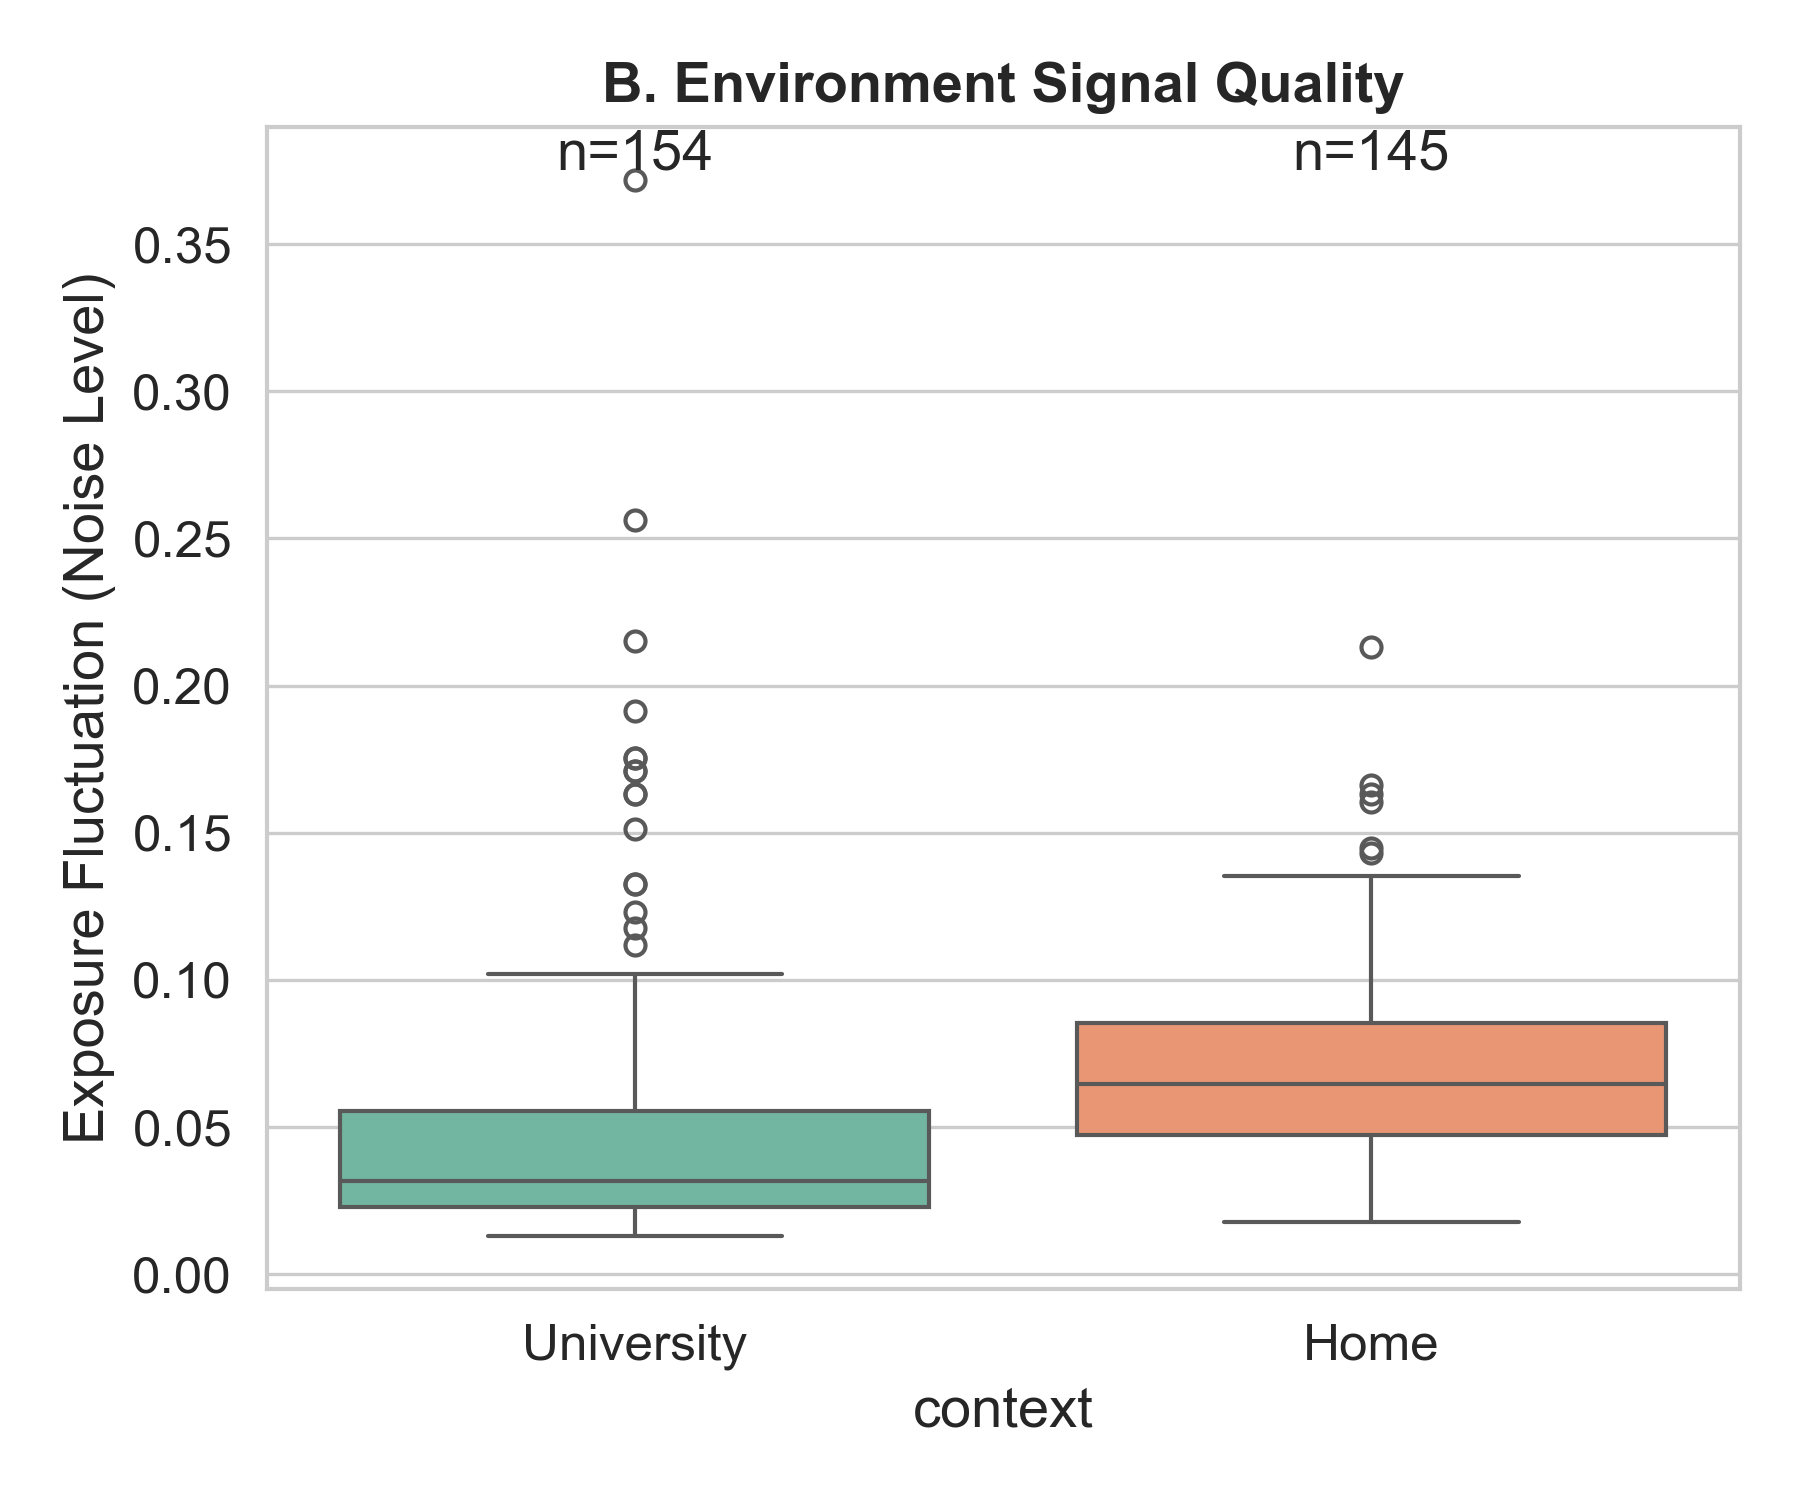
\includegraphics[width=\linewidth]{paper_figures/Figure2_Quality.png}
%DIFDELCMD <     %%%
%DIFDELCMD < \caption{%
{%DIFAUXCMD
\DIFdelFL{Data Quality Comparison. The Home environment (Orange) exhibits higher exposure fluctuation ($E_{fluc}$) and lower tracking confidence compared to the Laboratory (Blue), posing a challenge for rPPG signal extraction.}}
    %DIFAUXCMD
%DIFDELCMD < \label{fig:data_quality}
%DIFDELCMD < \end{center}
%DIFDELCMD < \end{figure}
%DIFDELCMD < 

%DIFDELCMD < \begin{table*}[t!]
%DIFDELCMD <     %%%
%DIFDELCMD < \caption{%
{%DIFAUXCMD
\DIFdelFL{Descriptive Data Quality Comparison (Trial-Level Aggregation)}}
%DIFAUXCMD
%DIFDELCMD < \label{tab:data_quality}
%DIFDELCMD < \begin{center}
%DIFDELCMD <     \resizebox{0.65\textwidth}{!}{%
%DIFDELCMD <     \begin{tabular}{lcc}
%DIFDELCMD < \toprule
%DIFDELCMD < \textbf{Metric (Mean $\pm$ SD)} & \textbf{Lab (292 trials)} & \textbf{Home (290 trials)} \\ 
%DIFDELCMD < \midrule
%DIFDELCMD < Frames per Second (FPS) & $59.8 \pm 0.4$ & $58.2 \pm 2.1$ \\
%DIFDELCMD < Face Size (IOD in px) & $142 \pm 12$ & $135 \pm 18$ \\
%DIFDELCMD < Mean Luminance (Y) & $180 \pm 15$ & $110 \pm 45$ \\
%DIFDELCMD < Exposure Fluctuation ($E_{fluc}$) & $0.03 \pm 0.01$ & $0.09 \pm 0.04$ \\
%DIFDELCMD < Tracking Conf. (\%) & $99.1\%$ & $96.5\%$ \\
%DIFDELCMD < \bottomrule
%DIFDELCMD < \end{tabular}
%DIFDELCMD <     }
%DIFDELCMD < \end{center}
%DIFDELCMD < \end{table*}
%DIFDELCMD < 

%DIFDELCMD < %%%
\DIFdel{The "Exposure Fluctuation" ($E_{fluc}$) was noticeably higher in the Home environment on average, indicating a difference in environmental lighting artifacts.
Despite this, the tracking confidence remained above 96\% at home , supporting the feasibility of using the MediaPipe + WebAssembly stack for this naturalistic deployment.
}%DIFDELCMD < 

%DIFDELCMD < %%%
\subsection{\DIFdel{Observation of Task Performance Differences}}
%DIFAUXCMD
\addtocounter{subsection}{-1}%DIFAUXCMD
\DIFdel{To investigate RQ2 (between-environment differences ), we aggregated Reaction Time (RT) across the three instructional framing conditions (Neutral, Negative Evaluation, Positive Evaluation) in both the Laboratory and Home environments.
We summarize trial-level variation descriptively to examine whether coarse between-environment differences were observable in this exploratory dataset}\DIFdelend \DIFaddbegin \DIFadd{the brightness-change indicator between settings.
These differences are treated as deployment-specific sensor-derived observations}\DIFaddend .

\DIFdelbegin %DIFDELCMD < \begin{figure}[t]
%DIFDELCMD <     \begin{center}
%DIFDELCMD <     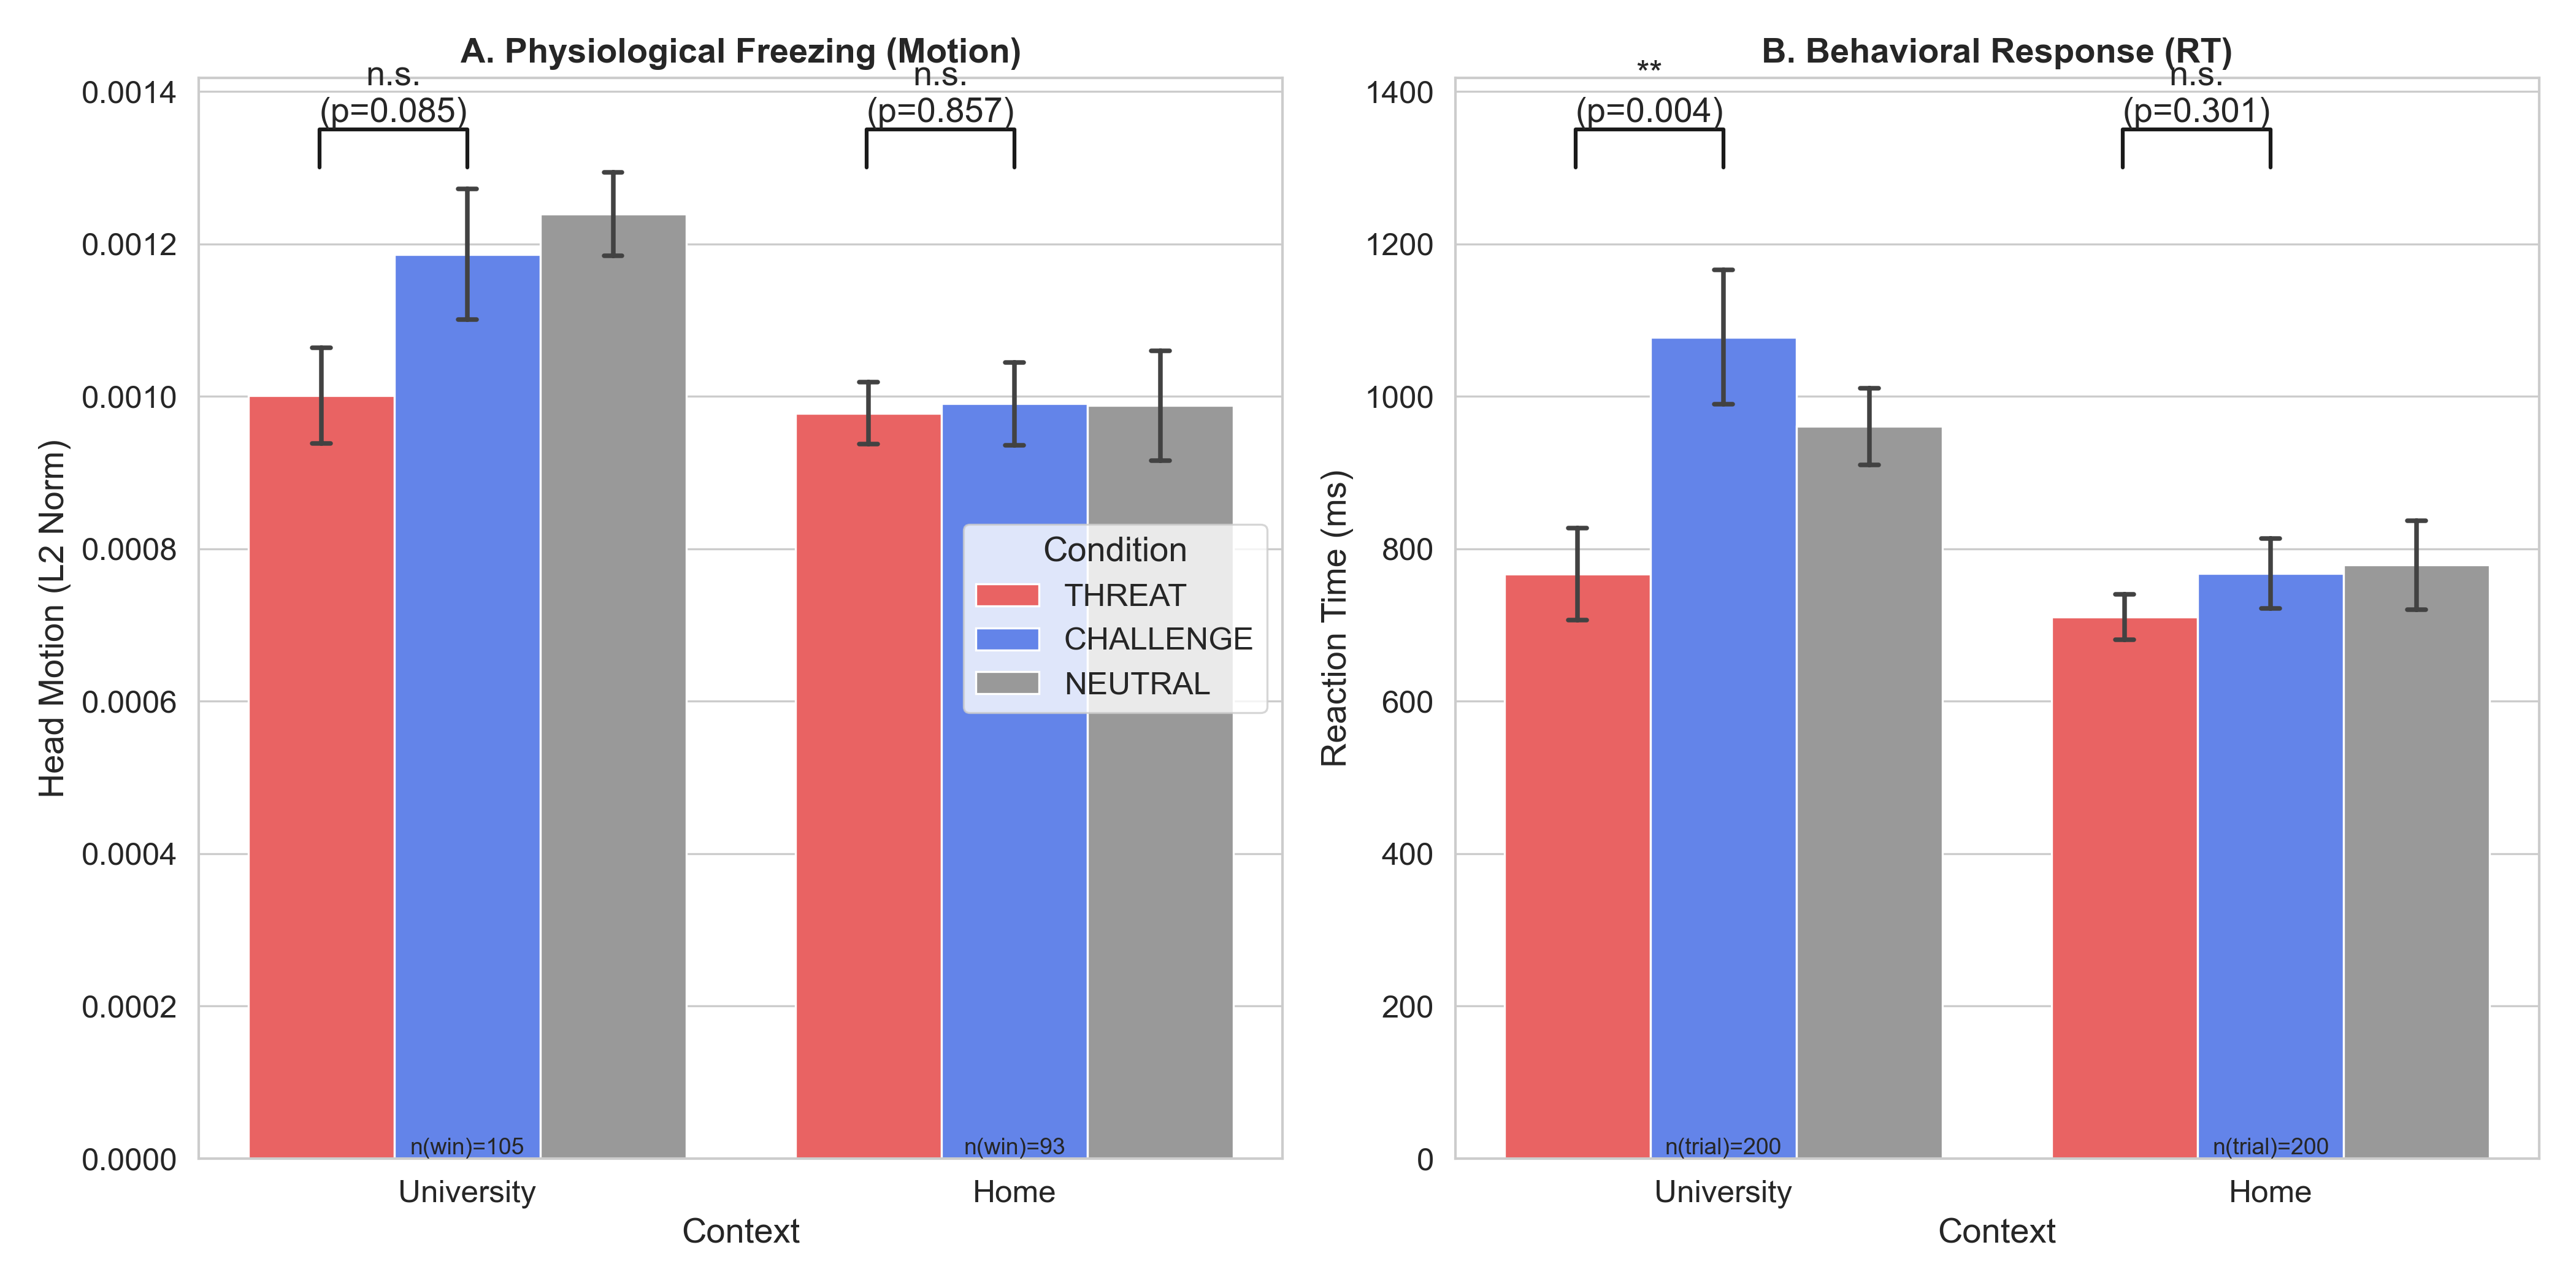
\includegraphics[width=\linewidth]{paper_figures/Figure3_Interaction.png}
%DIFDELCMD <     %%%
\DIFdelendFL \DIFaddbeginFL \begin{table*}[t]
\centering
\DIFaddendFL \caption{Descriptive \DIFdelbeginFL \DIFdelFL{trends in Reaction Time (RT) grouped by framing condition}\DIFdelendFL \DIFaddbeginFL \DIFaddFL{task and exported feature summaries after reaction-time exclusion}\DIFaddendFL .\DIFdelbeginFL \DIFdelFL{Under controlled Laboratory settings, the negative instructional framing exhibited descriptive deviations from the Neutral condition. At Home, variance across conditions appeared to mask task-induced deviations. Error bars represent Standard Error (SE).}\DIFdelendFL }
\DIFdelbeginFL %DIFDELCMD < \label{fig:rt_results}
%DIFDELCMD < \end{center}
%DIFDELCMD < \end{figure}
%DIFDELCMD < %%%
\DIFdelend \DIFaddbegin \label{tab:data_quality}
\footnotesize
\begin{tabular}{@{}p{0.30\textwidth}p{0.18\textwidth}p{0.18\textwidth}p{0.24\textwidth}@{}}
\toprule
\textbf{\DIFadd{Metric}} & \textbf{\DIFadd{Laboratory}} & \textbf{\DIFadd{Home}} & \textbf{\DIFadd{Notes}} \\
\midrule
\DIFadd{Retained trials after RT exclusion }& \DIFadd{256/300 (85.3\%) }& \DIFadd{285/300 (95.0\%) }& \DIFadd{Trial-level; RT 100--1500 ms }\\
\DIFadd{Mean RT after RT exclusion }& \DIFadd{721.1 $\pm$ 257.7 ms }& \DIFadd{676.5 $\pm$ 249.5 ms }& \DIFadd{Trial-level retained trials }\\
\DIFadd{Accuracy after RT exclusion }& \DIFadd{85.5\% }& \DIFadd{82.1\% }& \DIFadd{Trial-level retained trials }\\
\DIFadd{rPPG-oriented ROI green-channel value }& \DIFadd{46.69 $\pm$ 6.80 }& \DIFadd{34.32 $\pm$ 2.72 }& \DIFadd{Window-level; windows.csv }\\
\DIFadd{Motion estimate }& \DIFadd{0.0011 $\pm$ 0.0005 }& \DIFadd{0.0010 $\pm$ 0.0004 }& \DIFadd{Window-level; windows.csv }\\
\DIFadd{Frame-to-frame green-channel brightness-change indicator }& \DIFadd{0.0504 $\pm$ 0.0509 }& \DIFadd{0.0707 $\pm$ 0.0337 }& \DIFadd{Window-level; windows.csv }\\
\bottomrule
\end{tabular}
\end{table*}
\DIFaddend 

\DIFdelbegin \subsubsection{\DIFdel{Laboratory Environment}}
%DIFAUXCMD
\addtocounter{subsubsection}{-1}%DIFAUXCMD
\DIFdel{In the controlled Lab environment, the Negative Evaluation condition exhibited an observable acceleration in mean responses ($M = 485ms, SD = 82$) relative to the Neutral condition ($M = 520ms, SD = 95$) }\DIFdelend \DIFaddbegin \subsection{\DIFadd{Task-Event and Sensor-Derived Observations}}
\DIFadd{To address RQ2, we compared descriptive task-event and sensor-derived summaries across instructional task contexts and deployment contexts.
The exported logs showed descriptive differences in head-motion estimates and RT across laboratory and home contexts.
These differences should be interpreted as observations from this author-participant deployment, not as evidence that the instruction blocks induced psychological or motivational effects}\DIFaddend .
\DIFdelbegin \DIFdel{This pattern indicates that the task-derived response metric was more clearly separated from the neutral condition in the laboratory setting.}\DIFdelend 

\DIFdelbegin \subsubsection{\DIFdel{Home Environment}}
%DIFAUXCMD
\addtocounter{subsubsection}{-1}%DIFAUXCMD
\DIFdel{Conversely, in the Home environment, RTs across all conditions clustered closely around the Neutral condition (Negative: $M = 512ms$; Neutral: $M = 515ms$).
The descriptive separation observed in the laboratory setting was not apparent in the home setting.
This highlights the susceptibility of specific task-derived metrics to masking by uncontrolled domestic noise factors.
}\DIFdelend \DIFaddbegin \DIFadd{In the laboratory context, the negative instruction block showed a lower mean RT than the neutral block in this dataset.
In the home context, the mean RT values across instruction blocks were closer together.
Because the deployment used one author-participant and did not isolate instruction effects from environment, lighting, posture, or camera factors, these RT patterns are reported only as descriptive task-event observations.
}\DIFaddend 

\DIFdelbegin \subsection{\DIFdel{Between-Environment Differences in Physiological Features}}
%DIFAUXCMD
\addtocounter{subsection}{-1}%DIFAUXCMD
\DIFdel{We further investigated if differences extended to the collected physiological estimates.
}%DIFDELCMD < 

%DIFDELCMD < %%%
\subsubsection{\DIFdel{Head Motion}}
%DIFAUXCMD
\addtocounter{subsubsection}{-1}%DIFAUXCMD
\DIFdel{We analyzed the descriptive Head Motion Index ($M_t$) during the instruction-reading phase.
In the Lab, the Negative Evaluation condition showed a reduction in head motion compared to the Neutral condition.
At Home, however, higher motion variability was observed during the same instruction .
}%DIFDELCMD < 

%DIFDELCMD < %%%
\subsubsection{\DIFdel{Heart Rate Analysis (rPPG)}}
%DIFAUXCMD
\addtocounter{subsubsection}{-1}%DIFAUXCMD
\DIFdel{Due to the short trial duration (seconds per trial), we aggregated HR estimation across the entire block duration (approx.
2 minutes).
While the rPPG signal quality in the Lab provided clean peaks, the Home data suffered from noise artifacts during high-motion segments.
After excluding segments with high optical motion noise ($M_t > 2.0$), the observed }\DIFdelend \DIFaddbegin \subsection{\DIFadd{rPPG-Oriented ROI Estimates}}
\DIFadd{The exported data include rPPG-oriented ROI brightness values and related quality indicators, but no ECG or contact PPG reference was collected.
Therefore, this paper does not interpret ROI-derived or }\DIFaddend block-level \DIFdelbegin \DIFdel{descriptive differences were:
}%DIFDELCMD < \begin{itemize}
\begin{itemize}%DIFAUXCMD
%DIFDELCMD <     \item %%%
\item%DIFAUXCMD
\textbf{\DIFdel{Lab}}%DIFAUXCMD
\DIFdel{: The Negative Evaluation condition showed an average HR elevation of approximately $+8.5$ bpm relative to the Neutral condition.
}%DIFDELCMD < \item %%%
\item%DIFAUXCMD
\textbf{\DIFdel{Home}}%DIFAUXCMD
\DIFdel{: The same condition showed a mean HR change of $+1.2$ bpm.
}
\end{itemize}%DIFAUXCMD
%DIFDELCMD < \end{itemize}
%DIFDELCMD < %%%
\DIFdel{These physiological observations were reported alongside the task-derived trends and showed descriptive differences across environments}\DIFdelend \DIFaddbegin \DIFadd{summaries as validated heart-rate changes.
The appropriate interpretation is that the tested deployment yielded sensor-derived records whose values differed descriptively between the tested laboratory and home contexts}\DIFaddend .

% =================================================================================
% SECTION 6: DISCUSSION
% =================================================================================
\section{Discussion}

The \DIFdelbegin \DIFdel{central finding of this deployment is not a population-level effect of instructional framing, but that identical task procedures produced different observed task and physiological patterns across environments.
For system evaluation, this suggests that laboratory-only validation may overestimate signal stability and condition separability under domestic use.
This highlights an engineering constraint for continuous sensing: systems evaluated purely on Lab data may exhibit environment-associated changes in observed signals and measurement quality when moved from laboratory to domestic settings.
}\DIFdelend \DIFaddbegin \DIFadd{main implication of this work is system-design oriented.
Camerala illustrates how a browser-native runtime can combine task events, webcam-derived features, quality indicators, and local persistence without raw-video transmission in a remote task experiment conducted in laboratory and home settings.
The results do not establish general deployability, robustness, or physiological/cognitive effects.
Instead, they motivate design requirements and safeguards for future local-first deployments.
}\DIFaddend 

\DIFaddbegin \subsection{\DIFadd{Browser-Native Local-First Logging as a Design Pattern}}
\DIFadd{The useful system property demonstrated here is integration.
Task timing, frame-level feature extraction, quality indicators, and local export are handled in one client-side workflow.
This can reduce the need for raw-video handling and server-side timestamp reconciliation.
However, because raw video is not stored, researchers lose the ability to visually inspect many artifacts after data collection.
This trade-off makes quality-aware logging especially important.
}

\DIFaddend \subsection{\DIFdelbegin \DIFdel{Prioritizing Browser-Native Architectures}\DIFdelend \DIFaddbegin \DIFadd{Quality Indicators for Laboratory and Home Deployment Contexts}\DIFaddend }
\DIFdelbegin \DIFdel{Methodologically, we demonstrated that a browser-native framework (Camerala) can operationally collect synchronized behavioral and physiological data in domestic spaces without transmitting raw video.
By retaining computation purely on the client side, the architecture minimizes the privacy barriers that often inhibit exploratory "in-the-wild" deployments involving video sensors.
}\DIFdelend \DIFaddbegin \DIFadd{The deployment suggests that future systems should log not only task performance and rPPG-oriented estimates, but also indicators that help interpret the measurement pipeline.
Such indicators include landmark availability, rPPG-oriented ROI values, head-motion estimates, and camera-image-derived brightness-change records.
These values can support pre-session checks and descriptive inspection.
They should not be treated as proof that rPPG estimates are accurate.
}\DIFaddend 

\DIFaddbegin \subsection{\DIFadd{Interpreting Sensor-Derived Estimates Under Environmental Heterogeneity}}
\DIFadd{The laboratory/home differences should be interpreted cautiously because deployment context, lighting, posture, camera geometry, task timing, and participant state were not independently controlled.
The present design cannot isolate psychological, cognitive, motivational, or physiological effects.
They are better understood as deployment-specific sensor-derived observations under environmental heterogeneity.
Future work should include reference ECG or contact PPG, multiple participants, multiple devices, and controlled variation of environmental factors.
}

\subsection{\DIFadd{Design Safeguards for Future Camerala Deployments}}
\DIFadd{Future deployments should incorporate clearer safeguards: documented hardware/browser/camera settings, explicit reporting of camera constraints and actual camera settings, fixed screen-brightness settings, pre-session camera/lighting checks, landmark-availability warnings, camera-derived brightness-change records, and specified quality-aware analysis rules.
If privacy-sensitive raw video is not stored, these safeguards become more important because many artifacts cannot be retrospectively inspected from images.
For studies that aim to make claims about physiological responses, a reference physiological sensor and a multi-participant design are necessary.
}

\DIFaddend \subsection{Limitations}
\DIFdelbegin \DIFdel{There are several strict limitationsto this work}\DIFdelend \DIFaddbegin \DIFadd{This study has strict limitations}\DIFaddend .
First, \DIFdelbegin \DIFdel{this is a single-case exploratory deployment (}\DIFdelend \DIFaddbegin \DIFadd{it was an exploratory }\DIFaddend N=1 \DIFdelbegin \DIFdel{); the results represent observational, deployment-oriented feasibility evidence rather than generalizable population inference}\DIFdelend \DIFaddbegin \DIFadd{deployment with the author as participant}\DIFaddend .
Second, \DIFdelbegin \DIFdel{the observed between-environment differences in physiological signals do not definitively prove cognitive state changes; they may be heavily confounded by uncontrolled physical variables including ambient lightingchanges, subtle postureshifts, display luminescence, or camera placementartifacts inherent to unstructured deployments. Furthermore, the current work does not establish comparative superiority over existing runtimes or APIs. Future large-scale deployments must attempt to disentangle physical artifacts from cognitive shifts through sensor-fused studies.
Even with these limitations, }\DIFdelend \DIFaddbegin \DIFadd{there was no reference physiological sensor, ECG, or contact PPG.
Third, the deployment used one primary laptop/camera configuration and did not test multiple devices, multiple participants, or multiple home environments.
Fourth, lighting, posture, camera placement, and task context were not experimentally separated.
Fifth, no comparison with existing experiment runtimes, browser rPPG tools, or cloud APIs was conducted.
Sixth, the current logs do not store continuous confidence values from }\DIFaddend the \DIFdelbegin \DIFdel{present study establishes a concrete }\DIFdelend \DIFaddbegin \DIFadd{face-processing pipeline for all frames.
Therefore, failed landmark-detection frames and overall tracking-success rates cannot be recovered.
Future versions should log continuous confidence values for all frames and apply specified operational thresholds during analysis.
Seventh, the study does not claim clinical or medical accuracy, general deployability, general feasibility, robustness, or validated cognitive, motivational, psychological, or physiological effects.
The present study presents an implementation example of }\DIFaddend browser-native\DIFdelbegin \DIFdel{design pattern for privacy-conscious}\DIFdelend , task-aligned\DIFdelbegin \DIFdel{sensing under heterogeneous physical }\DIFdelend \DIFaddbegin \DIFadd{, local-first feature logging under limited laboratory and home }\DIFaddend conditions.

\section{Conclusion}
\DIFdelbegin \DIFdel{Continuous physiological sensing in naturalistic environments requires tools that balance operational stability with stringent privacy protections. }\DIFdelend We presented Camerala, a \DIFdelbegin \DIFdel{privacy-conscious}\DIFdelend \DIFaddbegin \DIFadd{browser-native}\DIFaddend , \DIFaddbegin \DIFadd{local-first framework that integrates psychophysical task execution, on-device rPPG/FaceMesh-derived feature extraction, measurement-quality indicators, and timestamped local persistence.
In a limited 10-session N=1 author-participant deployment across one laboratory setting and one home setting, the system completed 600 trials under the tested configuration without raw video transmission by Camerala.
After the specified reaction-time criterion, 541/600 trials remained for descriptive analysis.
The deployment produced synchronized behavioral logs and sensor-derived records, and it revealed descriptive differences between the tested environments.
These observations should not be interpreted as evidence of general deployability, robustness, or physiological/cognitive effects.
Instead, Camerala illustrates a task-aligned }\DIFaddend browser-native \DIFdelbegin \DIFdel{framework that extracts rPPGand facial landmarks on-device.
Our proof-of-concept deployment provided initial evidence of the framework's browser-native architecture and highlighted the degree to which heterogeneous physical environmentsare associated with changes in observed task and physiological signals.
These findings underscore the importance of evaluating sensor pipelines under domestic conditions and establish a concrete browser-native design pattern for synchronized, }\DIFdelend \DIFaddbegin \DIFadd{implementation and highlights design safeguards needed for future }\DIFaddend local-first physiological \DIFdelbegin \DIFdel{sensing under heterogeneous physical environments}\DIFdelend \DIFaddbegin \DIFadd{feature logging in home-based psychophysical experiments}\DIFaddend .

\section*{Data availability}
The dataset containing facial landmarks, \DIFdelbegin \DIFdel{extracted rPPG signals}\DIFdelend \DIFaddbegin \DIFadd{sensor-derived features}\DIFaddend , and behavioral responses associated with this study cannot be made publicly available due to privacy restrictions and potentially identifiable \DIFdelbegin \DIFdel{biological data originating from domestic (in-the-wild) recordings}\DIFdelend \DIFaddbegin \DIFadd{face-derived data from a domestic deployment context}\DIFaddend .

\section*{CRediT authorship contribution statement}
\textbf{Kotaro Furukawa}: Conceptualization, Methodology, Software, Investigation, Formal analysis, Writing - original draft.

\section*{Declaration of competing interest}
The \DIFdelbegin \DIFdel{authors declare that they have }\DIFdelend \DIFaddbegin \DIFadd{author declares that there are }\DIFaddend no known competing financial interests or personal relationships that could have appeared to influence \DIFdelbegin \DIFdel{the work reported in this paper}\DIFdelend \DIFaddbegin \DIFadd{this work}\DIFaddend .

\section*{Funding}
This work was supported by the College of Transdisciplinary Sciences for Innovation, Kanazawa University.

\DIFdelbegin \section*{\DIFdel{Declaration of generative AI and AI-assisted technologies in the manuscript preparation process}}
%DIFAUXCMD
\DIFdel{During the preparation of this work the author(s) used Google Gemini in order to refine the LaTeX code and format it according to the journal guidelines. After using this tool/service, the author(s)reviewed and edited the content as needed and take(s) full responsibility for the content of the published article.
}\DIFdelend \DIFaddbegin \begin{thebibliography}{99}
\DIFaddend 

\DIFdelbegin %DIFDELCMD < \begin{thebibliography}{1}
%DIFDELCMD < %%%
\DIFdelend \DIFaddbegin \bibitem{verkruysse2008}
\DIFadd{Wim Verkruysse, Lars~O. Svaasand, and J. Stuart Nelson.
}\newblock \DIFadd{Remote plethysmographic imaging using ambient light.
}\newblock {\em \DIFadd{Optics Express}}\DIFadd{, 16(26):21434--21445, 2008.
}\DIFaddend 

\DIFdelbegin \bibitem{wang_pos}
\DIFdel{Wenjin Wang, Albertus~C Den~Brinker, Sander Stuijk, and Gerard De~Haan. }\DIFdelend \DIFaddbegin \bibitem{poh_ica}
\DIFadd{Ming-Zher Poh, Daniel~J. McDuff, and Rosalind~W. Picard.
}\DIFaddend \newblock \DIFdelbegin \DIFdel{Algorithmic principles of remote ppg}\DIFdelend \DIFaddbegin \DIFadd{Non-contact, automated cardiac pulse measurements using video imaging and blind source separation}\DIFaddend .
\newblock {\em \DIFdelbegin \DIFdel{IEEE Transactions on Biomedical Engineering}\DIFdelend \DIFaddbegin \DIFadd{Optics Express}\DIFaddend }, \DIFdelbegin \DIFdel{64(7):1479--1491, 2016.
}\DIFdelend \DIFaddbegin \DIFadd{18(10):10762--10774, 2010.
}\DIFaddend 

\bibitem{deepphys}
Weixuan Chen and Daniel McDuff.
\newblock Deepphys: Video-based physiological measurement using convolutional attention networks.
\newblock In {\em Proceedings of the European Conference on Computer Vision (ECCV)}, pages 349--365, 2018.

\DIFdelbegin \bibitem{mcduff_rppg}
\DIFdel{Daniel McDuff and E~Blackford. }\DIFdelend \DIFaddbegin \bibitem{ayesha_web_vital}
\DIFadd{A.~H. Ayesha, D. Qiao, and F. Zulkernine.
}\DIFaddend \newblock \DIFdelbegin \DIFdel{Remote measurement of physiological responses: A review of recent
  advances. }\DIFdelend \DIFaddbegin \DIFadd{A web application for experimenting and validating remote measurement of vital signs.
}\DIFaddend \newblock \DIFaddbegin \DIFadd{In }\DIFaddend {\em \DIFdelbegin \DIFdel{ACM Transactions on Computing for Healthcare}\DIFdelend \DIFaddbegin \DIFadd{Information Integration and Web Intelligence (iiWAS 2022)}\DIFaddend }\DIFaddbegin \DIFadd{, Lecture Notes in Computer Science, vol. 13635, pages 237--251}\DIFaddend , \DIFdelbegin \DIFdel{1}\DIFdelend \DIFaddbegin \DIFadd{2022.
}\newblock \DIFadd{doi:10.1007/978-3-031-21047-1\_21.
}

\bibitem{labvanced_rppg}
\DIFadd{LabVanced.
}\newblock \DIFadd{Remote heart rate detection / rPPG.
}\newblock \url{https://www.labvanced.com/content/technology/en/remote-heart-rate-detection-rPPG/}\DIFadd{, accessed July 5, 2026.
}

\bibitem{facephys_demo}
\DIFadd{K. Wang.
}\newblock \DIFadd{FacePhys-Demo: Browser-based rPPG monitor with local inference.
}\newblock \url{https://github.com/KegangWangCCNU/FacePhys-Demo}\DIFadd{, accessed July 5, 2026.
}

\bibitem{rhythmedge}
\DIFadd{Z. Hasan, E. Dey, S.~R. Ramamurthy, N. Roy, and A. Misra.
}\newblock \DIFadd{Demo: RhythmEdge: Enabling contactless heart rate estimation on the edge.
}\newblock \DIFadd{In }{\em \DIFadd{2022 IEEE International Conference on Smart Computing (SMARTCOMP)}}\DIFadd{, pages 177--179, 2022.
}

\bibitem{gupta_privacy}
\DIFadd{D. Gupta and A. Etemad.
}\newblock \DIFadd{Privacy-preserving remote heart rate estimation from facial videos.
}\newblock \DIFadd{In }{\em \DIFadd{2023 IEEE International Conference on Systems, Man, and Cybernetics (SMC)}}\DIFadd{, pages 706--712, 2023.
}\newblock \DIFadd{doi:10.1109/SMC53992.2023.10394350.
}

\bibitem{di_lernia_rppg_wild}
\DIFadd{D. Di~Lernia, G. Finotti, M. Tsakiris, G. Riva, and M. Naber.
}\newblock \DIFadd{Remote photoplethysmography (rPPG) in the wild: Remote heart rate imaging via online webcams.
}\newblock {\em \DIFadd{Behavior Research Methods}}\DIFadd{, 56:6904--6914, 2024.
}\newblock \DIFadd{doi:10.3758/s13428-024-02398-0.
}

\bibitem{kooij_naber_open_rppg}
\DIFadd{K.~M. van der Kooij and M. Naber.
}\newblock \DIFadd{An open-source remote heart rate imaging method with practical apparatus and algorithms.
}\newblock {\em \DIFadd{Behavior Research Methods}}\DIFadd{, 51:2106--2119, 2019.
}\newblock \DIFadd{doi:10.3758/s13428-019-01256-8.
}

\bibitem{efficientphys}
\DIFadd{X. Liu, B. Hill, Z. Jiang, S. Patel, and D. McDuff.
}\newblock \DIFadd{EfficientPhys: Enabling simple, fast and accurate camera-based cardiac measurement.
}\newblock \DIFadd{In }{\em \DIFadd{Proceedings of the IEEE/CVF Winter Conference on Applications of Computer Vision (WACV)}}\DIFadd{, pages 5008--5017, 2023.
}

\bibitem{mobilephys}
\DIFadd{X. Liu, Y. Wang, S. Xie, X. Zhang, Z. Ma, D. McDuff, and S. Patel.
}\newblock \DIFadd{MobilePhys: Personalized mobile camera-based contactless physiological sensing.
}\newblock {\em \DIFadd{Proceedings of the ACM on Interactive, Mobile, Wearable and Ubiquitous Technologies}}\DIFadd{, 6}\DIFaddend (1)\DIFaddbegin \DIFadd{, 2022.
}\newblock \DIFadd{doi:10.1145/3517225.
}

\bibitem{rppg_toolbox}
\DIFadd{X. Liu, G. Narayanswamy, A. Paruchuri, X. Zhang, J. Tang, Y. Zhang, R. Sengupta, S. Patel, Y. Wang, and D. McDuff.
}\newblock \DIFadd{rPPG-Toolbox: Deep remote PPG toolbox.
}\newblock {\em \DIFadd{Advances in Neural Information Processing Systems}}\DIFadd{, 36, Datasets and Benchmarks Track, 2023.
}

\bibitem{bhutani_privacy_rppg}
\DIFadd{S. Bhutani, M. Elgendi, and C. Menon.
}\newblock \DIFadd{Preserving privacy and video quality through remote physiological signal removal.
}\newblock {\em \DIFadd{Communications Engineering}}\DIFadd{, 4}\DIFaddend :\DIFdelbegin \DIFdel{1--24, 2020.
}\DIFdelend \DIFaddbegin \DIFadd{66, 2025.
}\newblock \DIFadd{doi:10.1038/s44172-025-00363-z.
}\DIFaddend 

\DIFdelbegin \bibitem{barlow_sced}
\DIFdel{David~H Barlow, Matthew~K Nock, and Michel Hersen. }\DIFdelend \DIFaddbegin \bibitem{jspsych_joss}
\DIFadd{J.~R. de Leeuw, R.~A. Gilbert, and B. Luchterhandt.
}\DIFaddend \newblock \DIFaddbegin \DIFadd{jsPsych: Enabling an open-source collaborative ecosystem of behavioral experiments.
}\newblock \DIFaddend {\em \DIFdelbegin \DIFdel{Single case experimental designs:Strategies for studying
  behavior change}\DIFdelend \DIFaddbegin \DIFadd{Journal of Open Source Software}\DIFaddend }\DIFaddbegin \DIFadd{, 8(85):5351, 2023.
}\newblock \DIFadd{doi:10.21105/joss.05351}\DIFaddend .
\DIFaddbegin 

\bibitem{psychopy2}
\DIFadd{J.~W. Peirce, J.~R. Gray, S. Simpson, M. MacAskill, R. Hoechenberger, H. Sogo, E. Kastman, and J.~K. Lindelov.
}\DIFaddend \newblock \DIFdelbegin \DIFdel{Pearson, 3rd edition, 2009.
}\DIFdelend \DIFaddbegin \DIFadd{PsychoPy2: Experiments in behavior made easy.
}\newblock {\em \DIFadd{Behavior Research Methods}}\DIFadd{, 51:195--203, 2019.
}\newblock \DIFadd{doi:10.3758/s13428-018-01193-y.
}\DIFaddend 

\DIFdelbegin \bibitem{mediapipe_paper}
\DIFdel{Camillo Lugaresi, Tang Jiu, Matthias Grundmann, Chris Rubinstein, Fan Jensen,
  Vivek Kwatro, }\DIFdelend \DIFaddbegin \bibitem{mediapipe_framework}
\DIFadd{C. Lugaresi, J. Tang, H. Nash, }\DIFaddend et~al.
\newblock \DIFdelbegin \DIFdel{Mediapipe}\DIFdelend \DIFaddbegin \DIFadd{MediaPipe}\DIFaddend : A framework for building perception pipelines.
\newblock \DIFdelbegin %DIFDELCMD < {\em %%%
\DIFdel{arXivpreprint arXiv}\DIFdelend \DIFaddbegin \DIFadd{arXiv}\DIFaddend :1906.08172\DIFdelbegin %DIFDELCMD < }%%%
\DIFdelend , 2019.

\end{thebibliography}

\appendix{}
\subsection*{Supporting Example: Task Substitution}

A core engineering feature of the framework is the separation between task logic and the \DIFdelbegin \DIFdel{physiological extraction engine.
By standardizing the event logging interval around the }\texttt{\DIFdel{window.requestAnimationFrame}} %DIFAUXCMD
\DIFdel{target cycle, the framework is designed so that cognitive task logic can be replaced without modifying the MediaPipe vision thread. }\textbf{\DIFdel{Listing 1}} %DIFAUXCMD
\DIFdel{illustrates a pseudocode configuration for substituting the Gabor }\DIFdelend \DIFaddbegin \DIFadd{feature-extraction loop.
Listing 1 illustrates a simplified configuration for replacing the }\DIFaddend orientation task with a \DIFdelbegin \DIFdel{generalized Spatial Memory task block.
}\DIFdelend \DIFaddbegin \DIFadd{spatial-memory task while preserving the same logging pathway.
This example is intended to illustrate module separation rather than to provide additional validation data.
}\DIFaddend 

\vspace{3mm}
\noindent\footnotesize{\textbf{Listing 1:} Task substitution example}
\vspace{-1mm}
\begin{lstlisting}[basicstyle=\ttfamily\scriptsize, frame=single, language=JavaScript]
const task = {
  stimulus: renderSpatialGrid(memory_load_target),
  allowed_keys: ["Space"],
  on_frame_sync: (timestamp_ms) => {
    camerala_logger.logEvent("stimulus_onset", timestamp_ms);
  }
};
\end{lstlisting}
\vspace{2mm}

\DIFdelbegin \DIFdel{To provide a supporting example of this separation, the structure ensures that time-critical physiological measurements continue asynchronously, while semantic trial events (e.g., }\textit{\DIFdel{stimulus\_onset}}%DIFAUXCMD
\DIFdel{) are dynamically injected into the timeline. }\textbf{\DIFdel{Listing 2}} %DIFAUXCMD
\DIFdel{shows the resulting unified data stream where event markers coexist with dense sensor vectors}\DIFdelend \DIFaddbegin \DIFadd{Listing 2 shows a schema-style example of a local tabular log in which task events and frame-derived features can coexist through timestamps}\DIFaddend .

\vspace{3mm}
\noindent\DIFdelbegin %DIFDELCMD < \footnotesize{\textbf{Listing 2:} JSONL log example}
%DIFDELCMD < %%%
\DIFdelend \DIFaddbegin \footnotesize{\textbf{Listing 2:} Example local log schema}
\DIFaddend \vspace{-1mm}
\DIFdelbegin %DIFDELCMD < \begin{lstlisting}[basicstyle=\ttfamily\tiny, frame=single, language=json]
%DIFDELCMD < %%%
%DIF < DIFVRB {"time_ms": 4015.2, "event": "grid_on", "load": 4, "rppg_g": 110.4, "mot_x": 0.02}
%DIF < DIFVRB {"time_ms": 4016.8, "event": "frame_sync", "load": 4, "rppg_g": 109.8, "mot_x": 0.02}
%DIF < DIFVRB {"time_ms": 4032.5, "event": "frame_sync", "load": 4, "rppg_g": 111.1, "mot_x": 0.01}
%DIF < DIFVRB {"time_ms":4211.4,"event":"response","key":"Space","rt_ms":196.2,"rppg_g":112.0}
\DIFdelend \DIFaddbegin \DIFmodbegin
\begin{lstlisting}[basicstyle=\ttfamily\tiny, frame=single, language=csv,alsolanguage=DIFcode]
%DIF > time_ms,event,load,rppg_roi,head_motion
%DIF > 4015.2,grid_on,4,110.4,0.02
%DIF > 4016.8,frame_sync,4,109.8,0.02
%DIF > 4032.5,frame_sync,4,111.1,0.01
%DIF > 4211.4,response,4,112.0,0.01
\end{lstlisting}
\DIFmodend
\vspace{2mm}

\end{document}
